\documentclass[final]{lmuposter}
% helpful for justifying the boxes, use the following in the header:
%
\setlength{\parindent}{0pt}

% German language
%\usepackage[ngerman]{babel}
% Fonts of package UTF8
\usepackage[utf8x]{inputenc}

% pgf and tikz for graphics
\usepackage{pgf}
\usepackage{pgflibrarysnakes}
\usepackage{tikz}

% mathematical symbols of the ams package
\usepackage{amsmath}
\usepackage{amssymb}
\usepackage{bbm}

% supfigures
\usepackage{subfig}

% macros for vectors, matrix and so on
\newsavebox{\fmbox}
\newenvironment{fmpage}[1]
	{\begin{lrbox}{\fmbox}\begin{minipage}{#1}}
	{\end{minipage}\end{lrbox}\fbox{\usebox{\fmbox}}}
%
% Puts a algorithm environment
\newenvironment{algorithm}[1][]{%
	\begin{table}[h]
	\centering
	\begin{minipage}[t]{12cm}
	\hspace{\stretch{2}} {\caption{\label{#1} #1}}
	\rule[1.5ex]{12cm}{0.01cm}\\
	%\hspace{\stretch{2}} {\tiny \textsc{ #1}}}
	\hspace{\stretch{2}} \\
	% SPACE BEFORE \\ IS IMPORTANT, ELSE NO STRETCHING
	\vspace{-4ex}
	\begin{list}{#1}{\labelwidth=12em \leftmargin=120pt}
	\vspace{-1ex}
}{%
	\end{list}
	\rule[1ex]{12cm}{0.01cm}\\
	\end{minipage}
	\vspace{-2ex}
	\end{table}
}
%
\newcommand{\atem}[2]{\item[\texttt{#1}] #2\vspace{1ex}}
%
% Some math stuff, you need to include \usepackage{amsmath} 
%
%
%\mathop is needed to  get the spacing correct,
%
\newcommand{\sign}{\mathop{\mathrm{sign}}}
%
% greek symbols are displayed fat, too 
%
\renewcommand{\vector}[1]{\boldsymbol{#1}}
%
% use straight letters for matrixes
%
\renewcommand{\matrix}[1]{\mathbf{#1}}
%
% Some further definitions
%
\newcommand{\set}[1]{\mathbb{#1}}
\newcommand{\transpose}{\mathsf{T}}
\newcommand{\unity}{\mathbbm{1}}

\usepackage{MnSymbol}

% multicols package
\usepackage{multicol}
\usepackage{tabularx}
\usepackage{vwcol}  

% Python source code highlighting. Uses the listings package. Use lstinputlistings in the boxes of the
% poster.
% Python listing setup
\usepackage{color}
\usepackage[procnames]{listings}
\usepackage{setspace}
\renewcommand{\lstlistlistingname}{Code Listings}
\renewcommand{\lstlistingname}{Code Listing}
\definecolor{gray}{gray}{0.5}
\definecolor{lightgray}{gray}{0.9}
\definecolor{green}{rgb}{0,0.5,0}
\definecolor{lightgreen}{rgb}{0,0.7,0}
\definecolor{orange}{rgb}{1,0.5,0}
\definecolor{purple}{rgb}{0.5,0,0.5}
\definecolor{darkred}{rgb}{0.5,0,0}


\lstset{
language=python,
extendedchars=true,
%basicstyle=\ttfamily\small\setstretch{1},
basicstyle=\footnotesize,
mathescape=true,
breaklines=true,
numbers=left,
numbersep=10pt,
numberstyle=\tiny,
framexleftmargin=30pt,
xleftmargin=55pt,
stringstyle=\color{green},
showstringspaces=false,
alsoletter={1234567890},
otherkeywords={\ , \}, \{},
keywordstyle=\color{blue},
emph={access,and,as,break,class,continue,def,del,elif,else,%
except,exec,finally,for,from,global,if,import,in,is,%
lambda,not,or,pass,print,raise,return,try,while,assert},
emphstyle=\color{orange}\bfseries,
emph={[2]self},
emphstyle=[2]\color{gray},
emph={[4]ArithmeticError,AssertionError,AttributeError,BaseException,%
DeprecationWarning,EOFError,Ellipsis,EnvironmentError,Exception,%
False,FloatingPointError,FutureWarning,GeneratorExit,IOError,%
ImportError,ImportWarning,IndentationError,IndexError,KeyError,%
KeyboardInterrupt,LookupError,MemoryError,NameError,None,%
NotImplemented,NotImplementedError,OSError,OverflowError,%
PendingDeprecationWarning,ReferenceError,RuntimeError,RuntimeWarning,%
StandardError,StopIteration,SyntaxError,SyntaxWarning,SystemError,%
SystemExit,TabError,True,TypeError,UnboundLocalError,UnicodeDecodeError,%
UnicodeEncodeError,UnicodeError,UnicodeTranslateError,UnicodeWarning,%
UserWarning,ValueError,Warning,ZeroDivisionError,abs,all,any,apply,%
basestring,bool,buffer,callable,chr,classmethod,cmp,coerce,compile,%
complex,copyright,credits,delattr,dict,dir,divmod,enumerate,eval,%
execfile,exit,file,filter,float,frozenset,getattr,globals,hasattr,%
hash,help,hex,id,input,int,intern,isinstance,issubclass,iter,len,%
license,list,locals,long,map,max,min,object,oct,open,ord,pow,property,%
quit,range,raw_input,reduce,reload,repr,reversed,round,set,setattr,%
slice,sorted,staticmethod,str,sum,super,tuple,type,unichr,unicode,%
vars,xrange,zip},
emphstyle=[4]\color{purple}\bfseries,
morecomment=[s][\color{lightgreen}]{"""}{"""},
morekeywords={and,as,assert,break,class,continue,def,del,elif,else,except,
     finally,for,from,global,if,import,in,is,lambda,not,or,pass,print,
     return,try,while,with,yield},
commentstyle=\color{red}\slshape,
%literate={>>>}{\textbf{\textcolor{darkred}{>{>}>}}}3%
%         {...}{{\textcolor{gray}{...}}}3,
procnamekeys={def,class},
procnamestyle=\color{blue}\textbf,
%framexleftmargin=0mm, framextopmargin=0mm, frame=ovalbox,
backgroundcolor=\color{lightgray},
frame=single,
framerule=0pt,
}


% Python listing setup

\usepackage{color}
\usepackage[procnames]{listings}
\usepackage{textcomp}
\usepackage{setspace}
\usepackage[]{xcolor}
\definecolor{gray}{gray}{0.5}
\definecolor{green}{rgb}{0,0.5,0}
\definecolor{lightgreen}{rgb}{0,0.7,0}
\definecolor{purple}{rgb}{0.5,0,0.5}
\definecolor{darkred}{rgb}{0.7,0,0}

\lstnewenvironment{python}[1][]{
\lstset{
% Escape with funnyeyes.
escapeinside={(*@}{@*)},
language=python,
basicstyle=\ttfamily\small,
stringstyle=\color{green},
showstringspaces=false,
alsoletter={1234567890},
otherkeywords={\ , \}, \{},
keywordstyle=\color{blue},
emph={access,and,as,break,class,continue,def,del,elif,else,%
except,exec,finally,for,from,global,if,import,in, is,%
lambda,not,or,pass,print,raise,return,try,while,assert},
emphstyle=\color{orange}\bfseries,
emph={[2]self},
emphstyle=[2]\color{gray},
emph={[4]ArithmeticError,AssertionError,AttributeError,BaseException,%
DeprecationWarning,EOFError,Ellipsis,EnvironmentError,Exception,%
False,FloatingPointError,FutureWarning,GeneratorExit,IOError,%
ImportError,ImportWarning,IndentationError,IndexError,KeyError,%
KeyboardInterrupt,LookupError,MemoryError,NameError,None,%
NotImplemented,NotImplementedError,OSError,OverflowError,%
PendingDeprecationWarning,ReferenceError,RuntimeError,RuntimeWarning,%
StandardError,StopIteration,SyntaxError,SyntaxWarning,SystemError,%
SystemExit,TabError,True,TypeError,UnboundLocalError,UnicodeDecodeError,%
UnicodeEncodeError,UnicodeError,UnicodeTranslateError,UnicodeWarning,%
UserWarning,ValueError,Warning,ZeroDivisionError,abs,all,any,apply,%
basestring,bool,buffer,callable,chr,classmethod,cmp,coerce,compile,%
complex,copyright,credits,delattr,dict,dir,divmod,enumerate,eval,%
execfile,exit,file,filter,float,frozenset,getattr,globals,hasattr,%
hash,help,hex,id,input,int,intern,isinstance,issubclass,iter,len,%
license,list,locals,long,map,max,min,object,oct,open,ord,pow,property,%
quit,range,raw_input,reduce,reload,repr,reversed,round,set,setattr,%
slice,sorted,staticmethod,str,sum,super,tuple,type,unichr,unicode,%
vars,xrange,zip},
emphstyle=[4]\color{purple}\bfseries,
upquote=true,
morecomment=[s][\color{lightgreen}]{"""}{"""},
commentstyle=\color{red}\slshape,
literate={>>>}{\bfseries{\textcolor{darkred}{>{>}>}}}3%
         {...}{{\textcolor{gray}{...}}}3,
procnamekeys={def,class},
procnamestyle=\color{blue}\textbf,
framexleftmargin=1mm, framextopmargin=1mm,
rulesepcolor=\color{blue},#1
}}{}



% Bibliography.
\usepackage[numbers,sort&compress, square]{natbib}
%
% Remove the bibliography header.
%
\makeatletter
\renewenvironment{thebibliography}[1]{%
%     \section*{\refname}%
%      \@mkboth{\MakeUppercase\refname}{\MakeUppercase\refname}%
      \list{\@biblabel{\@arabic\c@enumiv}}%
           {\settowidth\labelwidth{\@biblabel{#1}}%
            \leftmargin\labelwidth
            \advance\leftmargin\labelsep
            \@openbib@code
            \usecounter{enumiv}%
            \let\p@enumiv\@empty
            \renewcommand\theenumiv{\@arabic\c@enumiv}}%
      \sloppy
      \clubpenalty4000
      \@clubpenalty \clubpenalty
      \widowpenalty4000%
      \sfcode`\.\@m}
     {\def\@noitemerr
       {\@latex@warning{Empty `thebibliography' environment}}%
      \endlist}
\makeatother

% some modifications for the lists environment
%\renewcommand{\labelitemii}{$\blacktriangleright$}%
\setlength{\itemsep}{1mm}
\setlength{\parsep}{1mm}

\begin{document}
\nocite{obspy}


%\begin{tikzpicture}
%\node[left,text width=0.9\textwidth]at(0cm,0cm){ 
%\tiny
%\includegraphics[width=0.2\textwidth]{./images/obspy_logo_no_text_highres.png}\\[-3ex]
%};
%\end{tikzpicture}

%
% Document header
%
\PosterHead{
	%\textbf{\LARGE ObsPy: A Python Toolbox for Seismology/Seismological Observatories}\\[0.4ex]
	%\textit{\Large Interactive Application and Rapid Program Development} \\[0.5ex]
	%\large \underline{Lion Krischer}$^{\text{a}}$, Moritz Beyreuther$^{\text{a}}$, Robert Barsch$^{\text{a}}$, Tobias Megies$^{\text{a}}$, Yannik Behr$^{\text{b}}$, Joachim Wassermann$^{\text{a}}$\\
    \begin{center}
        %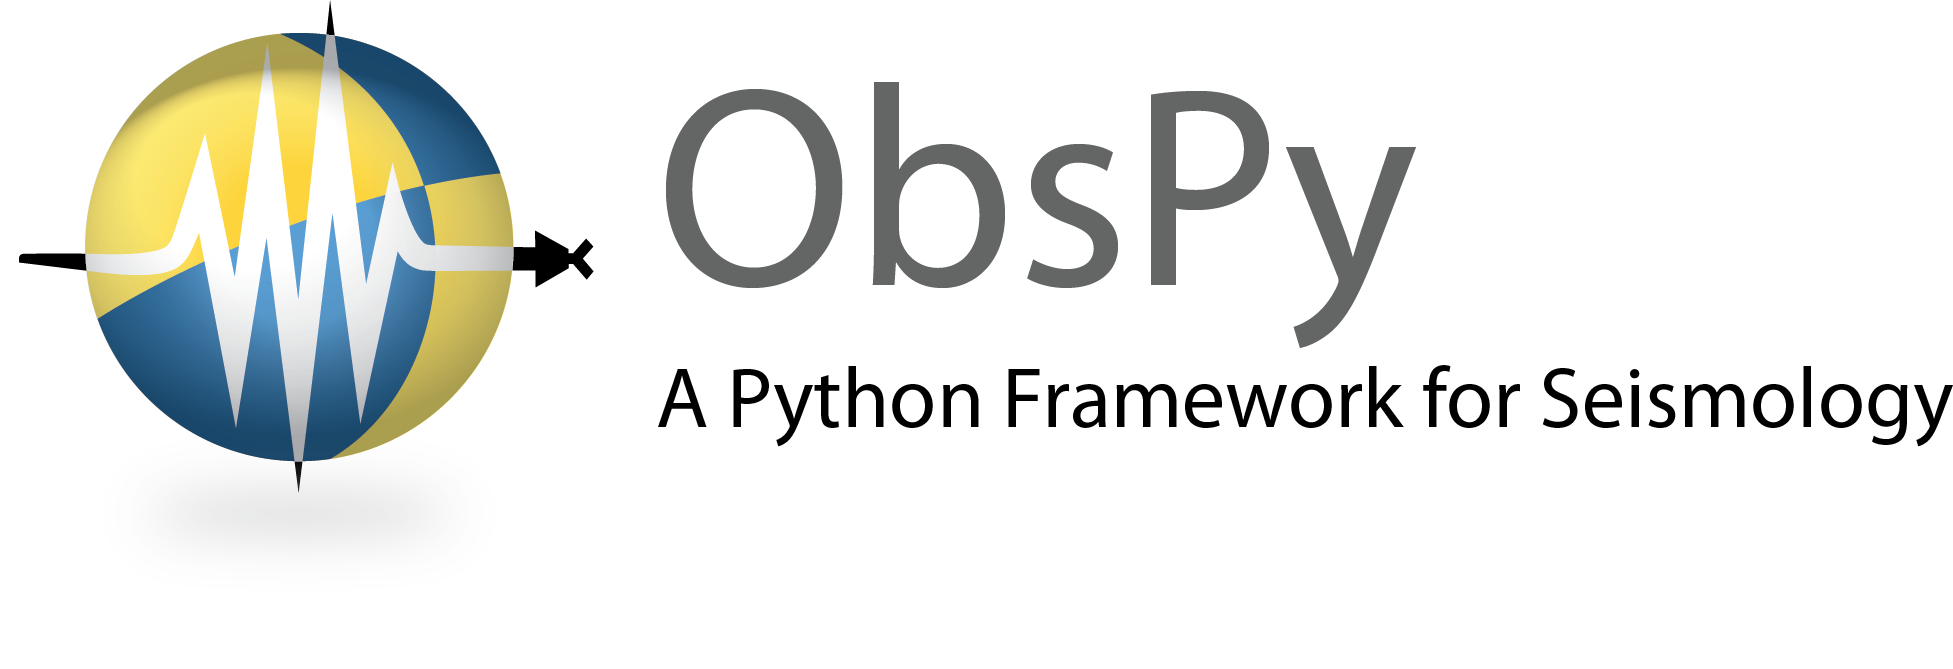
\includegraphics[width=0.5\columnwidth]{./images/obspy_logo_full_highres.png} \\
 %   \begin{vwcol}[widths={0.3,0.8},
  %           sep=.8cm, justify=flush,rule=0pt,indent=1em]
        %\includegraphics[width=0.25\columnwidth]{./images/obspy_logo_no_text_highres.png} \\
        %\newpage
    \vspace{3.4ex}
	\textbf{\LARGE ObsPy: A Python Toolbox for Seismology}\\[3.4ex]
    %\end{center}
    \large \textit{Tobias Megies, Lion Krischer, Robert Barsch, Moritz Beyreuther, Joachim Wassermann}\\
	%$^{\text{a}}$ LMU Munich \hspace{2em}  $^{\text{b}}$ Victoria University of Wellington, New Zealand\\
	Department of Earth and Environmental Sciences, Ludwig-Maximilians-University Munich, Germany\\
	Contact: \textit{devs@obspy.org} \textbf{https://www.obspy.org}
    \end{center}
%\end{vwcol}
}

%\begin{tikzpicture}[remember picture, overlay]
%\node [shift={(-1in,1in)}]  at (current page.center)
%{\fbox{\includegraphics[height=7.30in]{./images/obspy_logo_no_text_highres.png}}};
%\end{tikzpicture}

%
%\renewcommand{\capsize}{\footnotesize}
%
\setlength{\columnsep}{\MyBoxHSep}
\vspace{-1.5em}
\begin{multicols}{2}

%
% Left, first box.
%
\MyBox[8em]{
\section*{Summary}
\small
Python combines the power of a \textbf{full-blown programming language} with the
flexibility and fast code development of an \textbf{interactive scripting
language}. Its extensive standard library and large variety of freely available
high quality scientific modules cover most needs in \textbf{developing
scientific processing workflows}.

\textbf{ObsPy extends Python’s capabilities to fit the specific needs that
arise when working with seismological data.} It \textit{a)} provides
\textbf{read and write support for all of the most important waveform, station
and event metadata formats} \textit{b)} enables
\textbf{direct access to all important data centers, web services and
databases} to easily retrieve waveform data and station/event metadata and
\textit{c)} comes with a continuously growing \textbf{powerful signal
processing toolbox} that covers all every-day tasks in seismological analysis.

In combination with mature and free Python packages like NumPy, SciPy,
Matplotlib, IPython, Pandas and PyQt, \textbf{ObsPy makes it possible to
develop complete seismological processing workflows}, ranging
from reading locally stored data or requesting data from one or more different
data centers via signal analysis and data processing to visualization in GUI
and web applications, output of modified/derived data and the creation of
publication-quality figures.

All functionality is \textbf{extensively documented} and the online \textbf{ObsPy
Tutorial and Gallery} give a good impression of the wide range of possible use
cases. ObsPy is tested and \textbf{running on Linux, MacOS X and Windows} and
comes with installation routines for these systems. ObsPy is developed in a
test-driven approach and is available under the \textbf{LGPLv3 open source
licence}.

Users are welcome to request help, report bugs, propose enhancements or
contribute code via either the user mailing list or the \textbf{project page on
GitHub}.

\vspace{0.9em}
}\vspace{\MyBoxVSep}

\columnbreak%\\

%
% Right, first box.
%
\MyBox[8em]{
\small

\begin{multicols}{2}
\section*{Impact}
Six years after the beginnings of the project, ObsPy is used by
seismologists all around the world. With \textbf{more than 500 downloads for
Debian/Ubuntu Linux alone}, we estimate -- including Mac, Windows and other
Linux/Unix users -- an \textbf{active user base of around 1000-2000 people}.

Since ObsPy's start by a \textbf{core developer team of 3-5 people} at LMU Munich, ObsPy
has evolved into a community effort with \textbf{contributions to the code base
by 40 individuals}. The \textbf{percentage of contributions from outside the core
developer team is constantly on the rise and is currently at around 40\%}.

The user mailing list currently has over \textbf{300 subscribers} and serves as a
place for discussions and asking for help from more experienced users.

The \textbf{impact of ObsPy and the appreciation within the seismological
community} finds expression in the \textbf{rapidly increasing number of scientific
citations, which stands at over 70 as of October 2014}.
%\begin{itemize}
%    \item Around 25 people contributed code so far
%    \item Estimated active user base of \textbf{more than 5000} people
%    \item Code hosted on Github $\Rightarrow$ Anyone can contribute
%    \item Mature and stable code base
%    \item Stable development process
%    \item Runs everywhere
%    \item Goal: Built enough momentum for ObsPy to be self-sustainable
%\end{itemize}
%
%\vspace{2ex}
%
\columnbreak
\begin{center}
    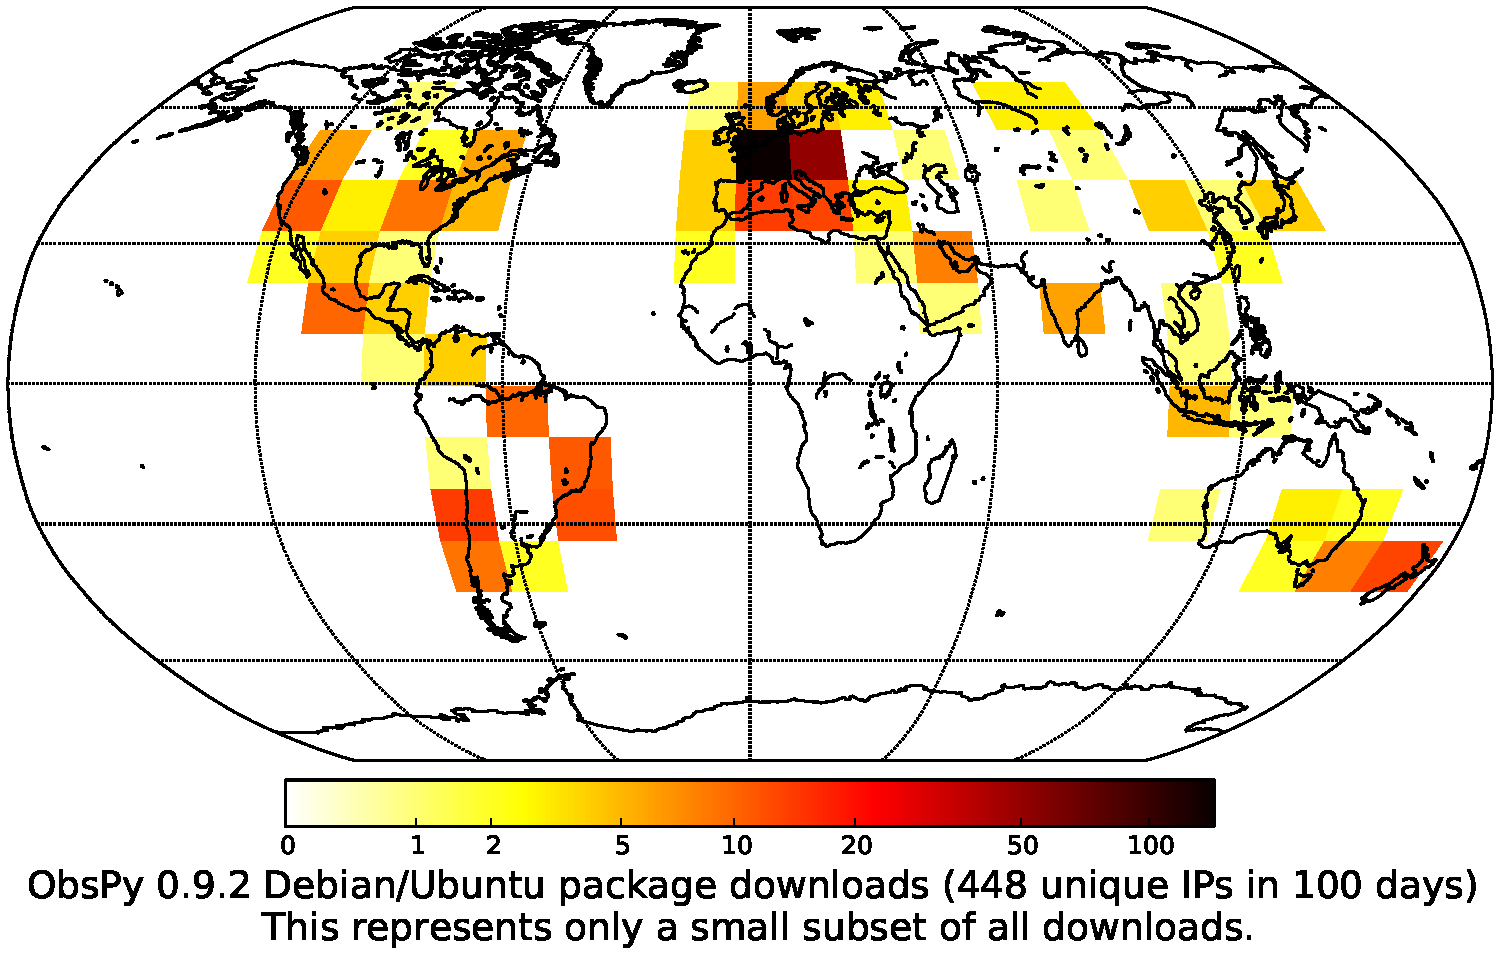
\includegraphics[width=0.8\columnwidth]{./images/obspy-deb.pdf} \\
\end{center}

\begin{center}
    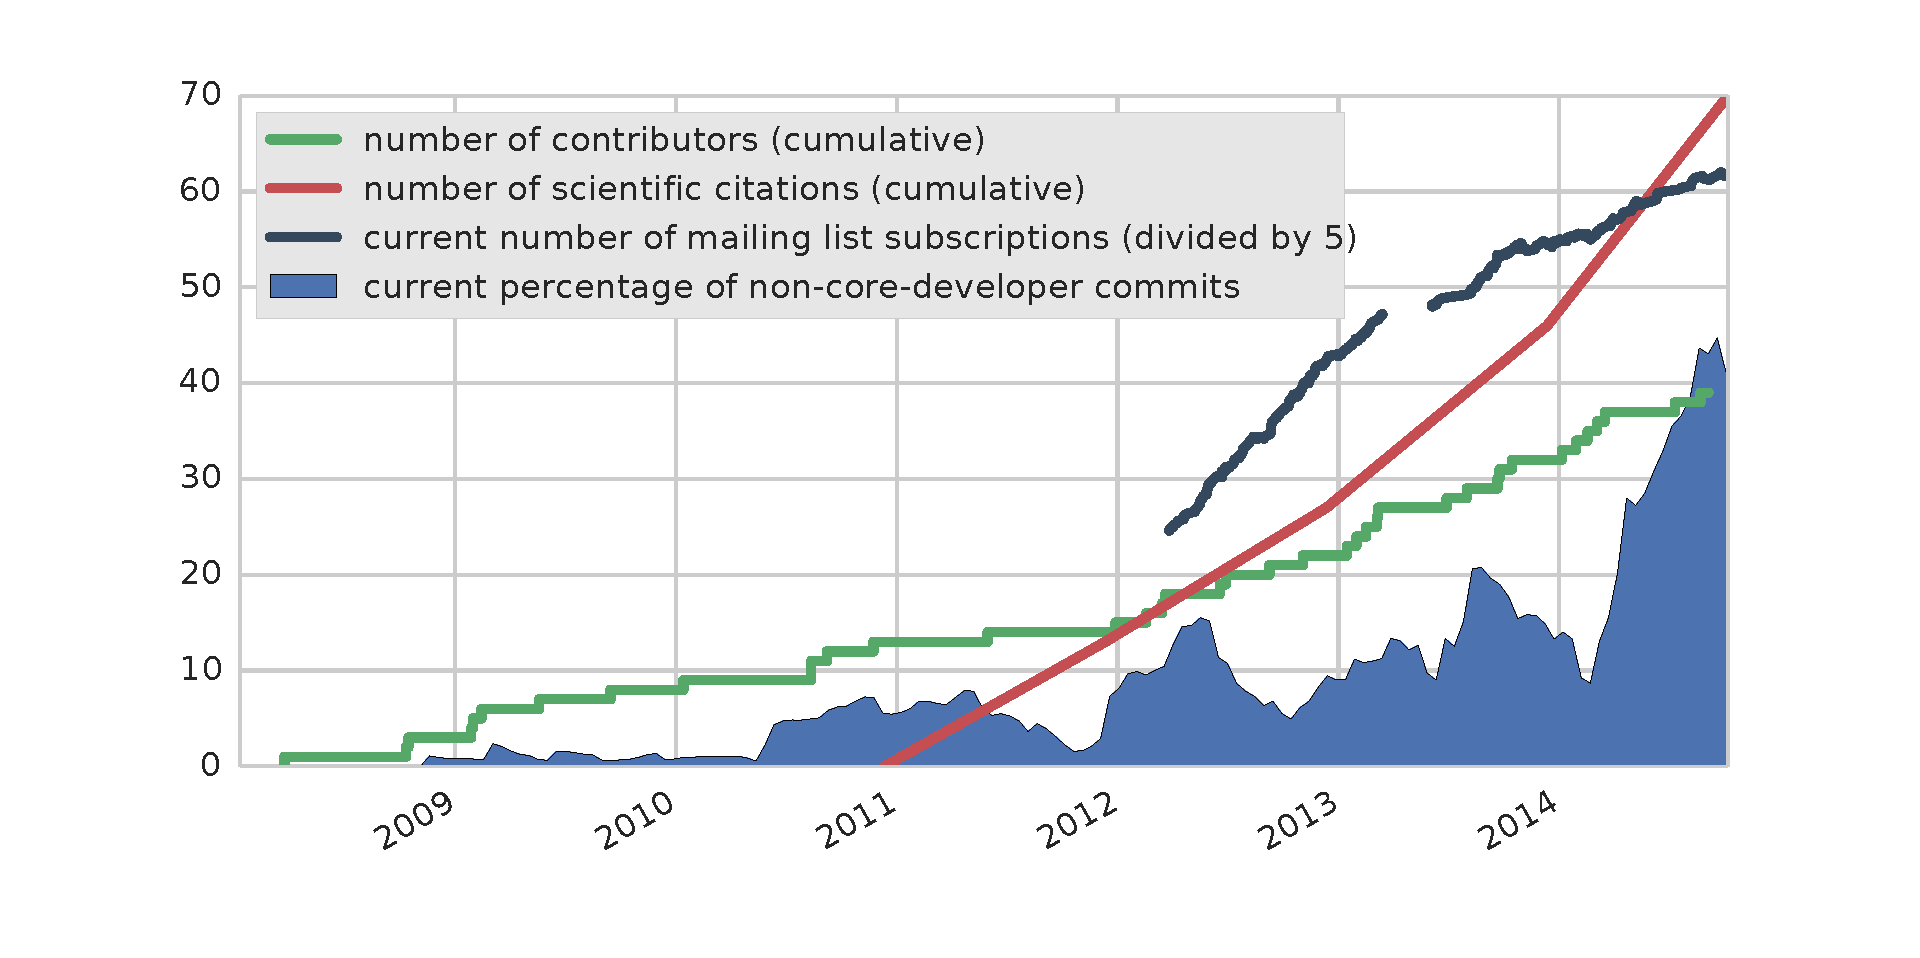
\includegraphics[width=1.0\columnwidth]{./images/all_stats.pdf} \\
\end{center}
\end{multicols}

}\vspace{\MyBoxVSep}

\end{multicols}

% First reduce the vertical spacing to zero and then expand again.
\vspace{-0.60cm}
\vspace{\MyBoxVSep}

% New width.
\setlength{\MyBoxWidth}{736.5mm}
%
% Full width box.
%
\MyBox[8em]{
\section*{Basic Example}
\footnotesize
\begin{multicols}{3}
\begin{center}
\begin{minipage}{\columnwidth}
\begin{python}^^J
from obspy import UTCDateTime^^J
from obspy.fdsn import Client^^J
^^J
# connect to LMU observatory web service^^J
client = Client("http://erde.geophysik.uni-muenchen.de:8080")^^J
^^J
# use origin time of devastating Japan earthquake^^J
start = UTCDateTime("2011-03-11 05:46:23") + 10 * 60^^J
end = start + 70 * 60^^J
^^J
# download waveform and station metadata of station FUR^^J
stream = client.get_waveforms(^^J
    network="GR", station="FUR", location="", channel="BH*",^^J
    starttime=start, endtime=end, attach_response=True)^^J
^^J
# do basic signal processing and plot the data!  ---->^^J
stream.remove_response()^^J
stream.filter("bandpass", freqmin=0.01, freqmax=1)^^J
stream.plot()^^J
\end{python}
%\begin{python}^^J
%>>> from obspy import read^^J
%>>> st = read("waveform.mseed")^^J
%>>> print st^^J
%1 Trace(s) in Stream:^^J
%BW.FURT..EHZ | 2010-01-04 ... | 200.0 Hz, 7204234 samples^^J
%>>> st[0].data^^J
%array([-426, -400, ... , -489, -339], dtype=int32)^^J
%>>> st.trim(endtime=st[0].stats.starttime + 3600)^^J
%>>> st.decimate(factor=2)^^J
%>>> st.filter("lowpass", freq=1.0)^^J
%>>> print st^^J
%BW.FURT..EHZ | 2010-01-05T ... | 100.0 Hz, 360001 samples^^J
%>>> st.plot()^^J
%\end{python}^^J
\end{minipage}
\end{center}
\columnbreak%\\
\begin{center}
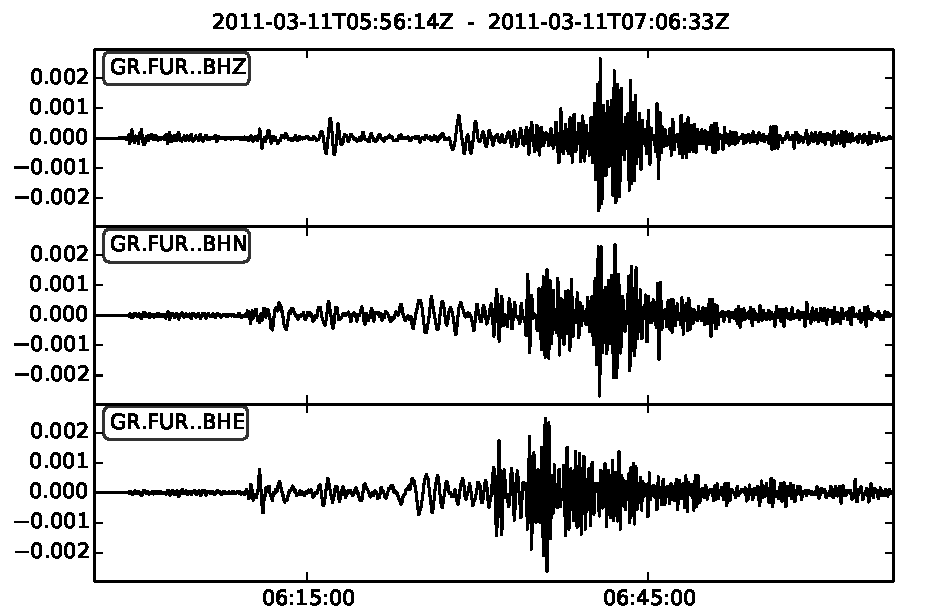
\includegraphics[width=0.85\columnwidth]{./images/obspy_example.pdf} \\
\end{center}
\columnbreak%\\
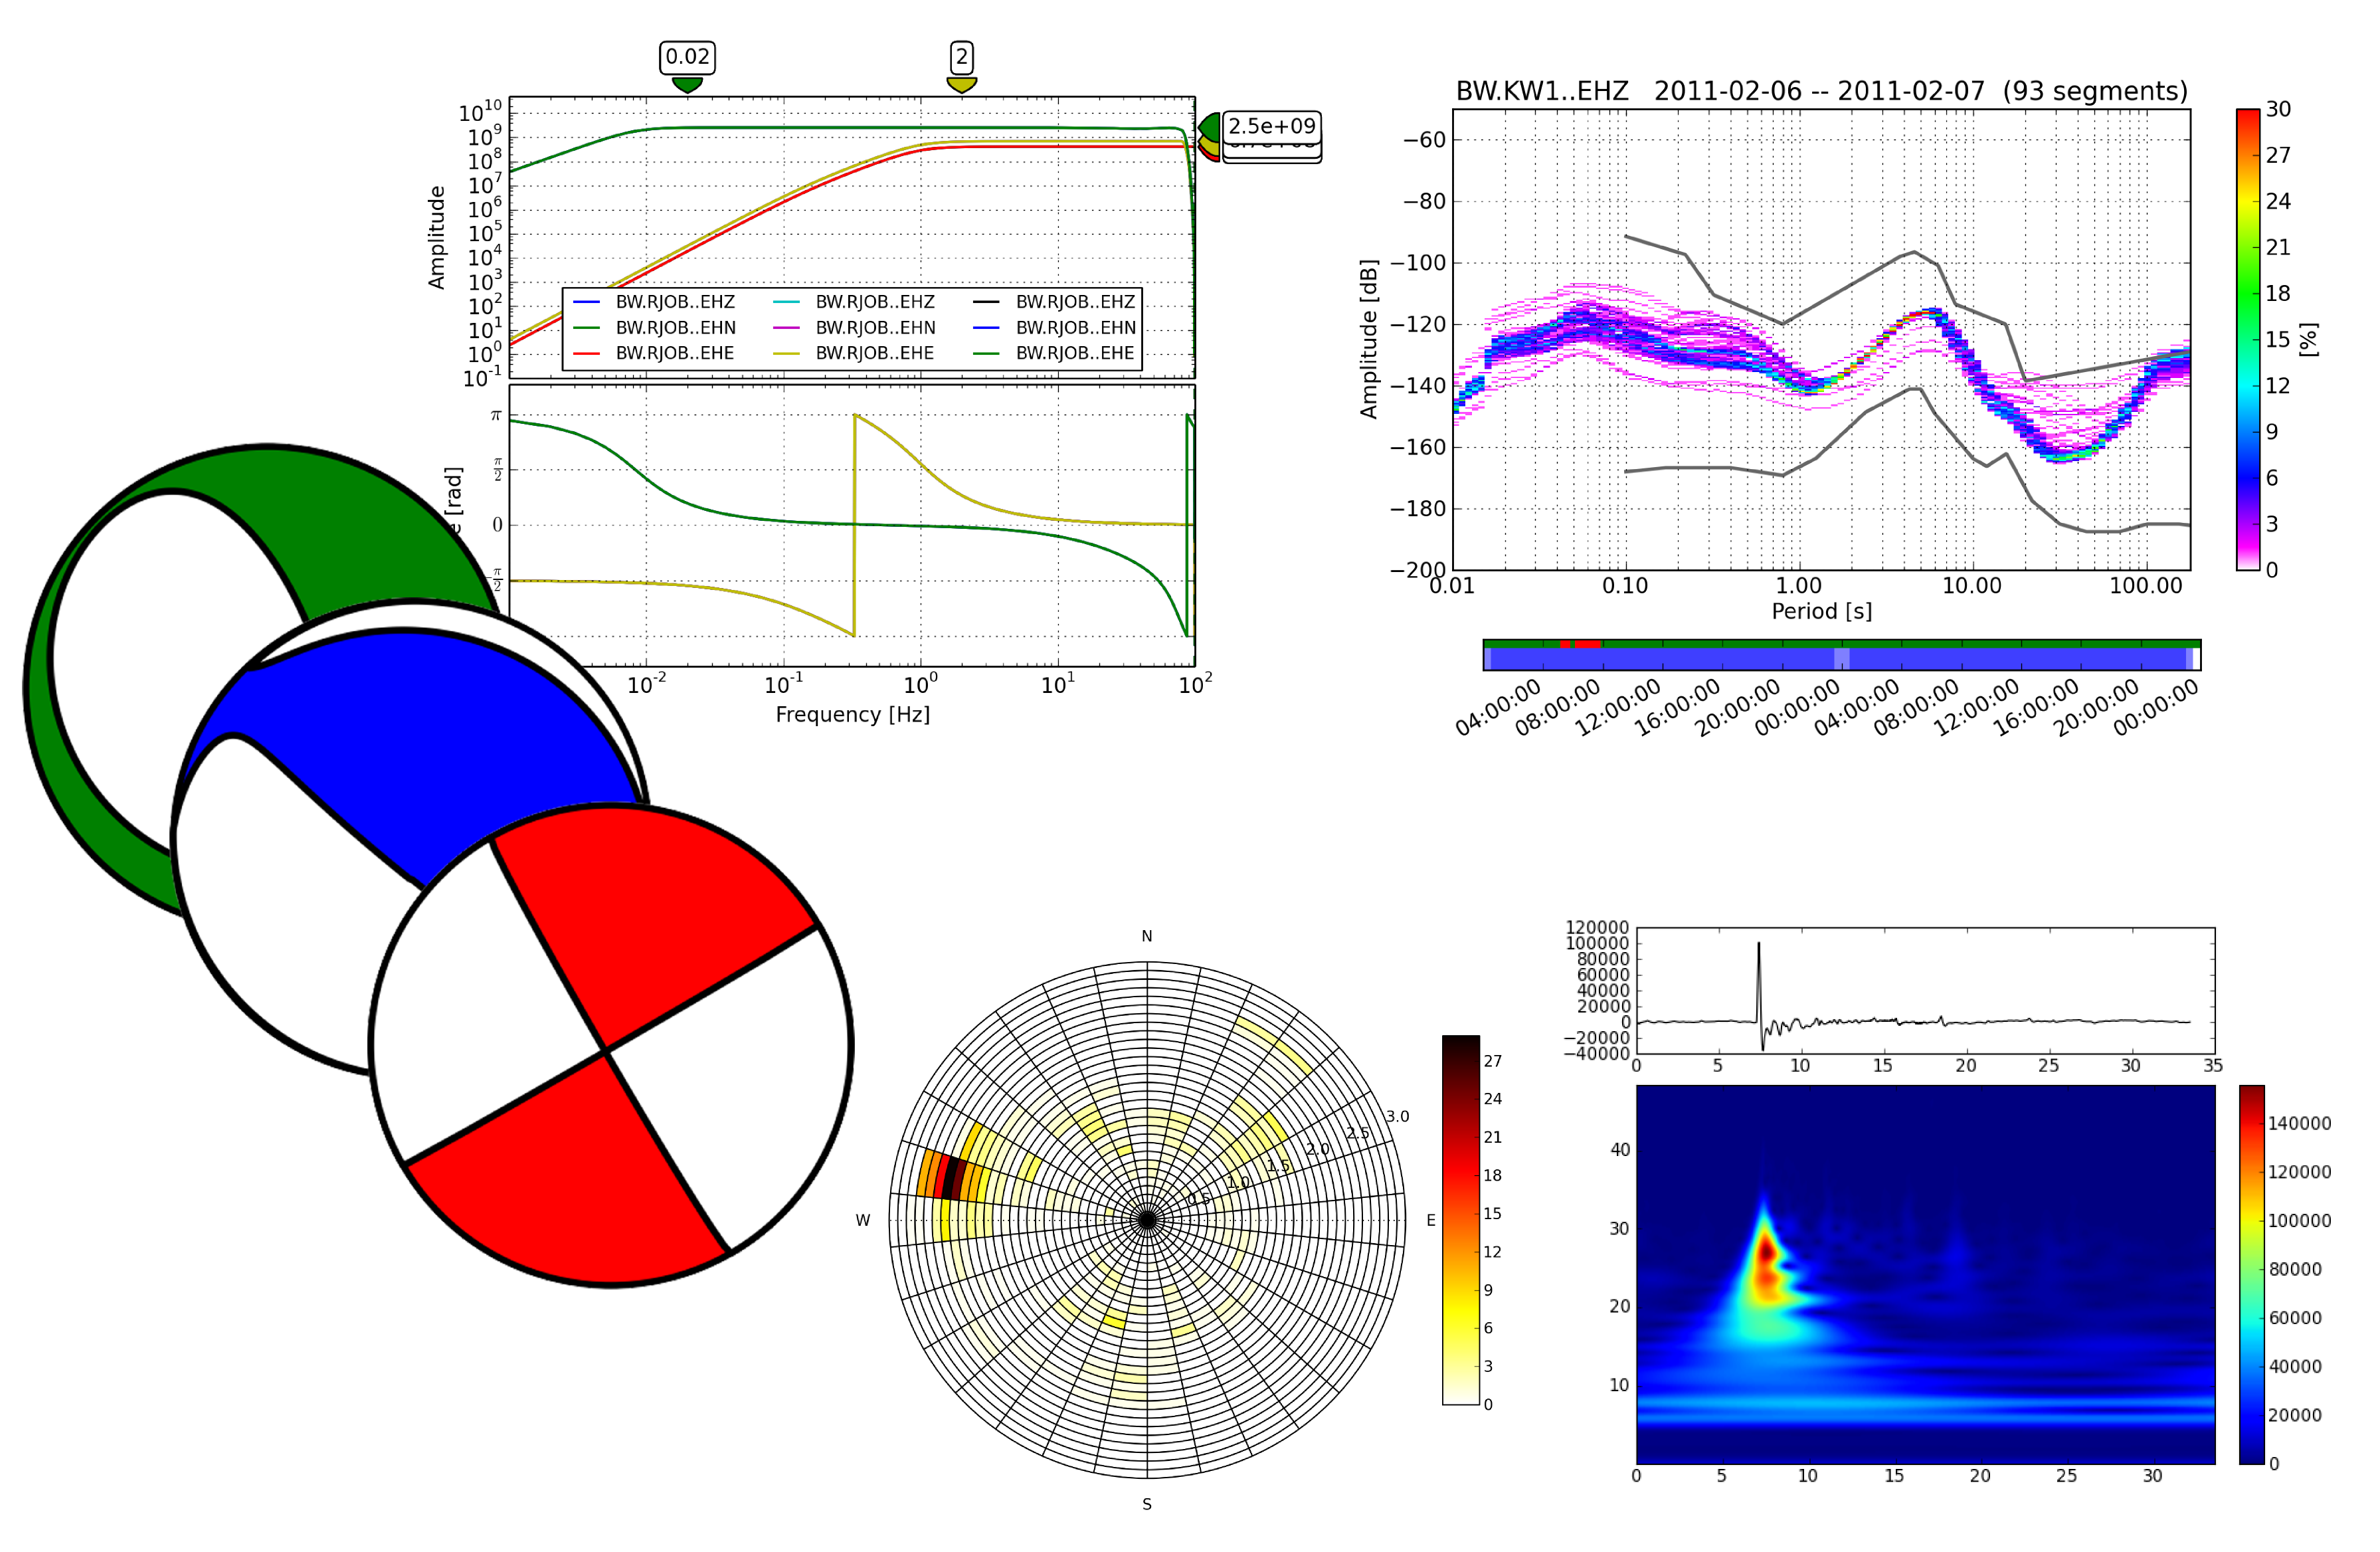
\includegraphics[width=0.85\columnwidth]{./images/collage.png} \\
\end{multicols}
}

\setlength{\MyBoxWidth}{355mm}
\begin{multicols}{2}
%
% Left, second box.
%
\MyBox[8em]{
%\section*{What Can ObsPy Do?}
\small
%\begin{itemize}
%    \item \textbf{Read and write waveform data in various formats} (MiniSEED, SAC, GSE, SEG Y, \dots) with a unified interface.
%    \item \textbf{Database and web service access clients} for the new FDSN web services, NERIES, IRIS DMC, ArcLink, SeisHub and Earthworm (experimental).
%    \item \textbf{Many seismological signal processing routines} like filters, trigger, instrument correction, array analysis, beamforming, \dots
%    \item \textbf{Support for inventory data} (SEED, XSEED, RESP, and StationXML support)
%    \item \textbf{Event data handling} (Supports the latest QuakeML 1.2 version)
%    \item \textbf{Unified time handling} Uses UTC $\Rightarrow$ No ambiguities
%\end{itemize}
%
%\begin{center}
%    +
%\end{center}
%
%\begin{center}
%    \textbf{The full power and flexibility of Python.}
%\end{center}
\section*{What Can I Do with ObsPy?}
\begin{multicols}{2}
Easy to use helper functions to access local files and online data centers give
\textbf{quick access to all data neccessary for seismological data analysis}.

All acquired information is exposed to
the user in \textbf{ObsPy's core classes that handle waveform data, station and event
metadata in a unified, consistent fashion, regardless of the data source}. This makes it easy to
combine data from different sources in unified workflows, both interactively and
automated.

ObsPy's core classes have many convenience routines for signal processing
directly attached for \textbf{quick, reproducible and well tested execution of
common processing tasks}.
\columnbreak
\begin{center}
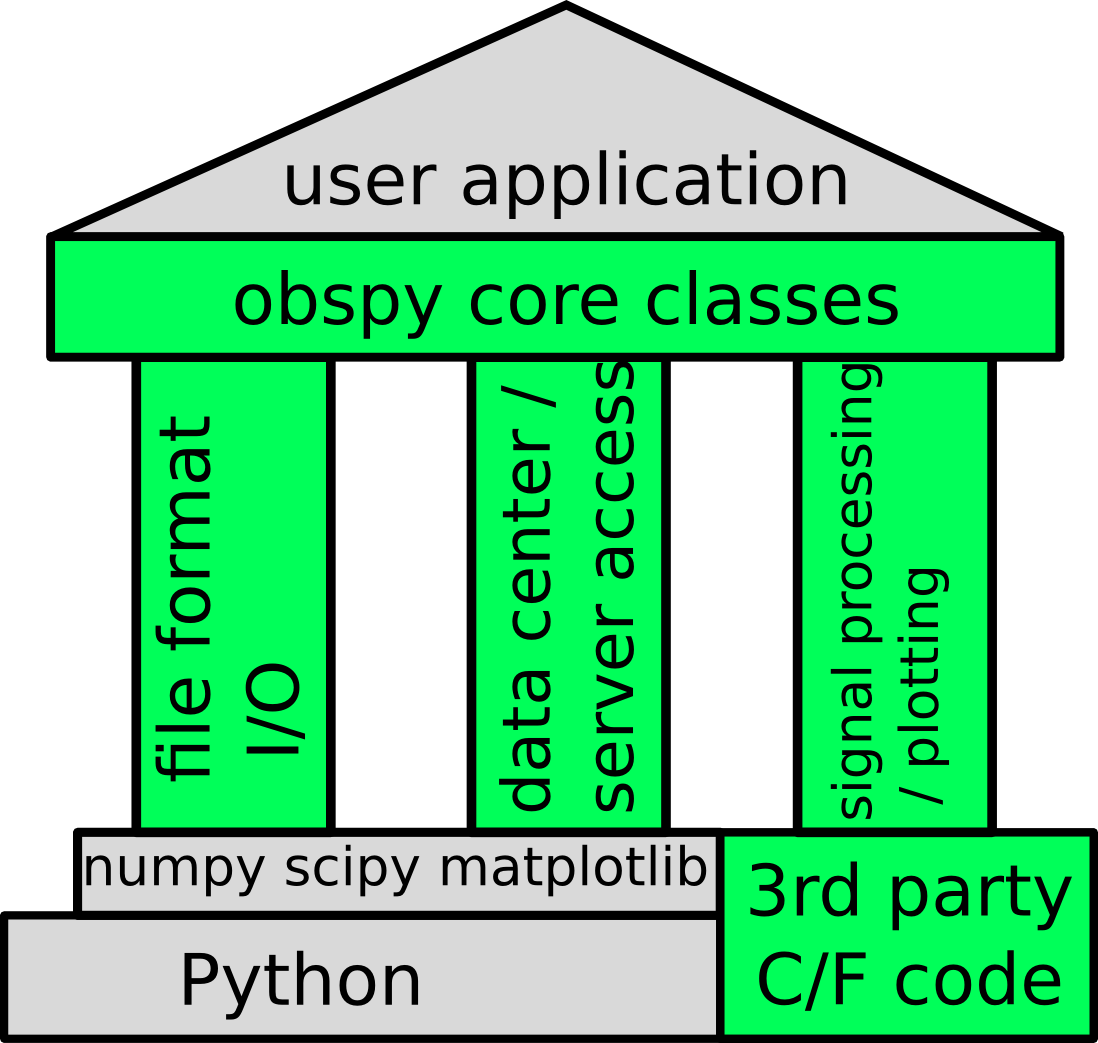
\includegraphics[width=0.65\columnwidth]{./images/obspy_pillars.png} \\
\end{center}
\end{multicols}
\vspace{\MyBoxVSep}

\begin{center}
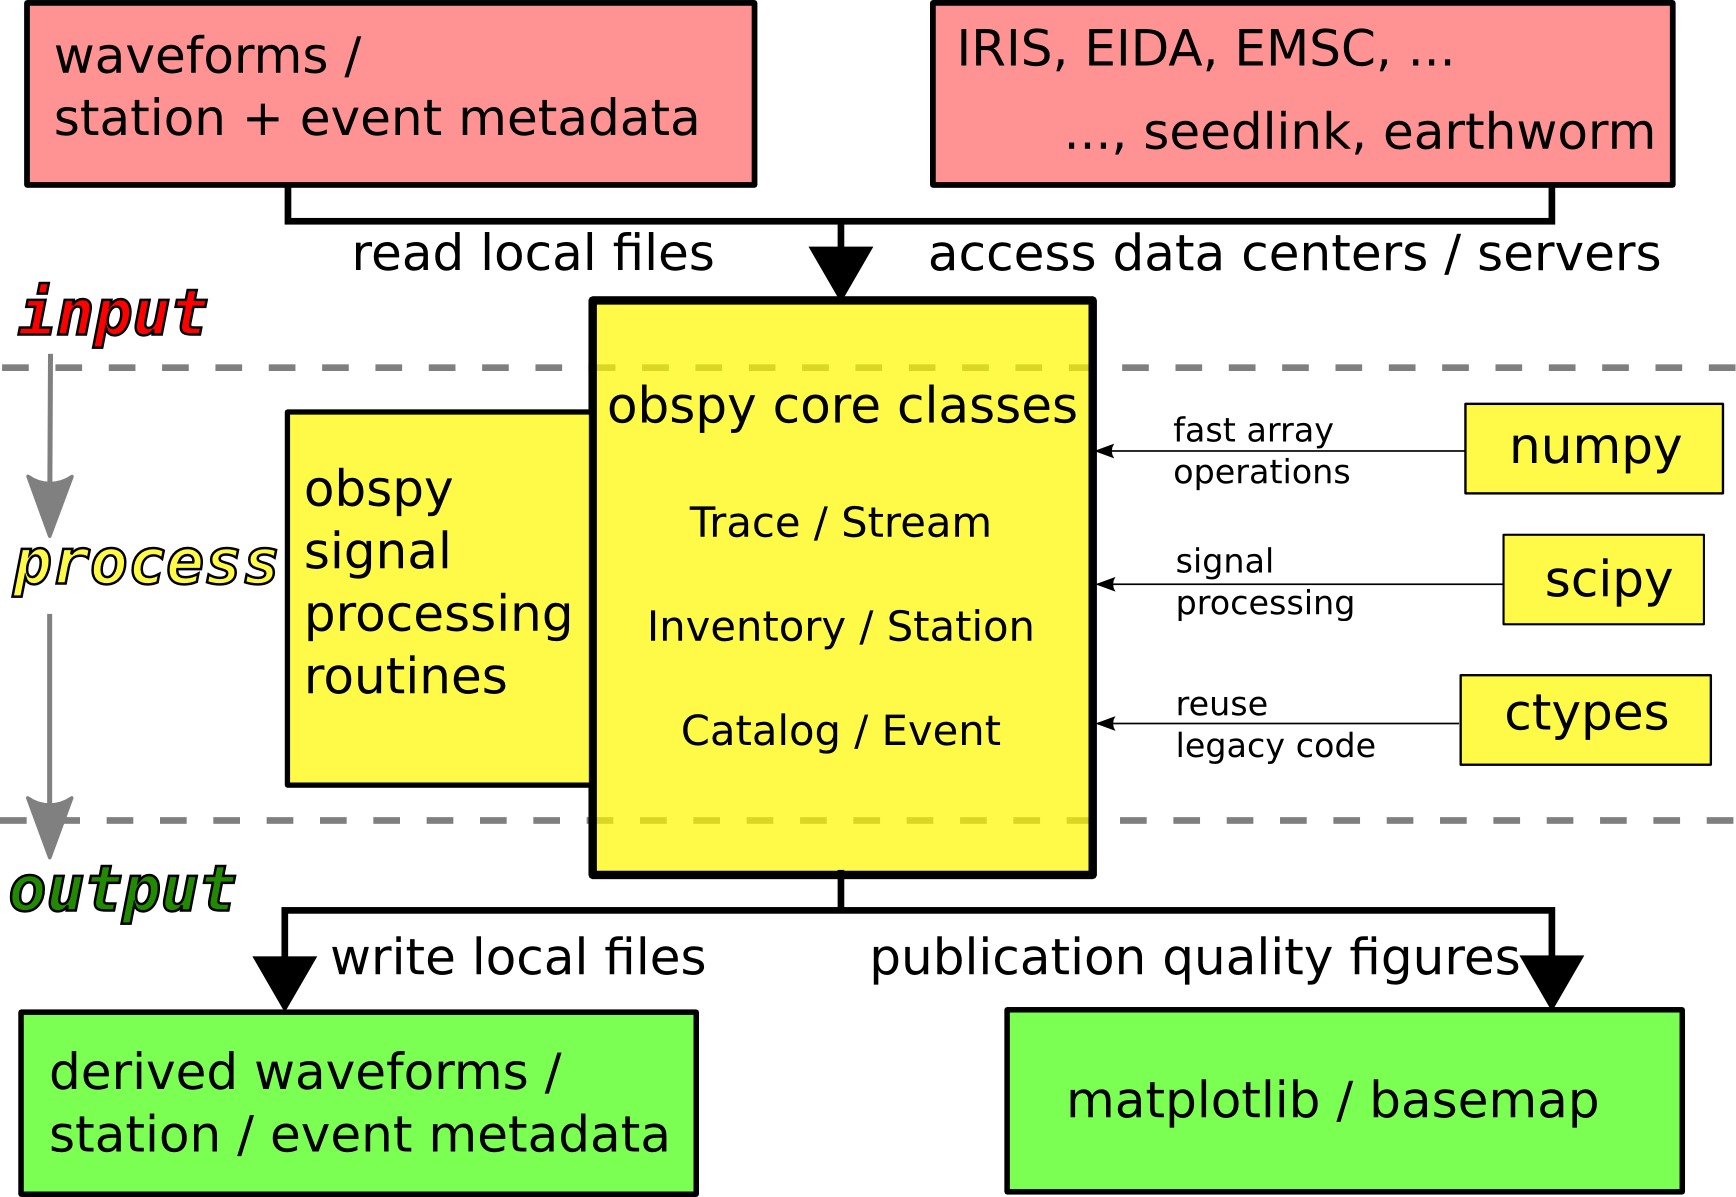
\includegraphics[width=0.764\columnwidth]{./images/obspy_workflow.png} \\
\end{center}

}\vspace{\MyBoxVSep}

\columnbreak

%
% Right, second box.
%
\MyBox[8em]{
\small


    \begin{center}
    \begin{tabularx}{\textwidth}{rX}
        \begin{minipage}{0.6\columnwidth}
\section*{ObsPy's Online Resources}
            \begin{itemize}
                \item Source Code, Bug Tracker, and Wiki
                \item Extensive documentation and example gallery
                \item Tutorial on how to get started
                \item \textbf{[obspy-users]} mailing list
                \item Installation Instructions for various platforms
                \item Use cases and user application showcases
            \end{itemize}
        \end{minipage}
        &
        \begin{minipage}{0.4\columnwidth}
            \begin{center}
%            \includegraphics[height=3cm]{./images/obspy-qr.png}
%
%            \vspace{3ex}
%
            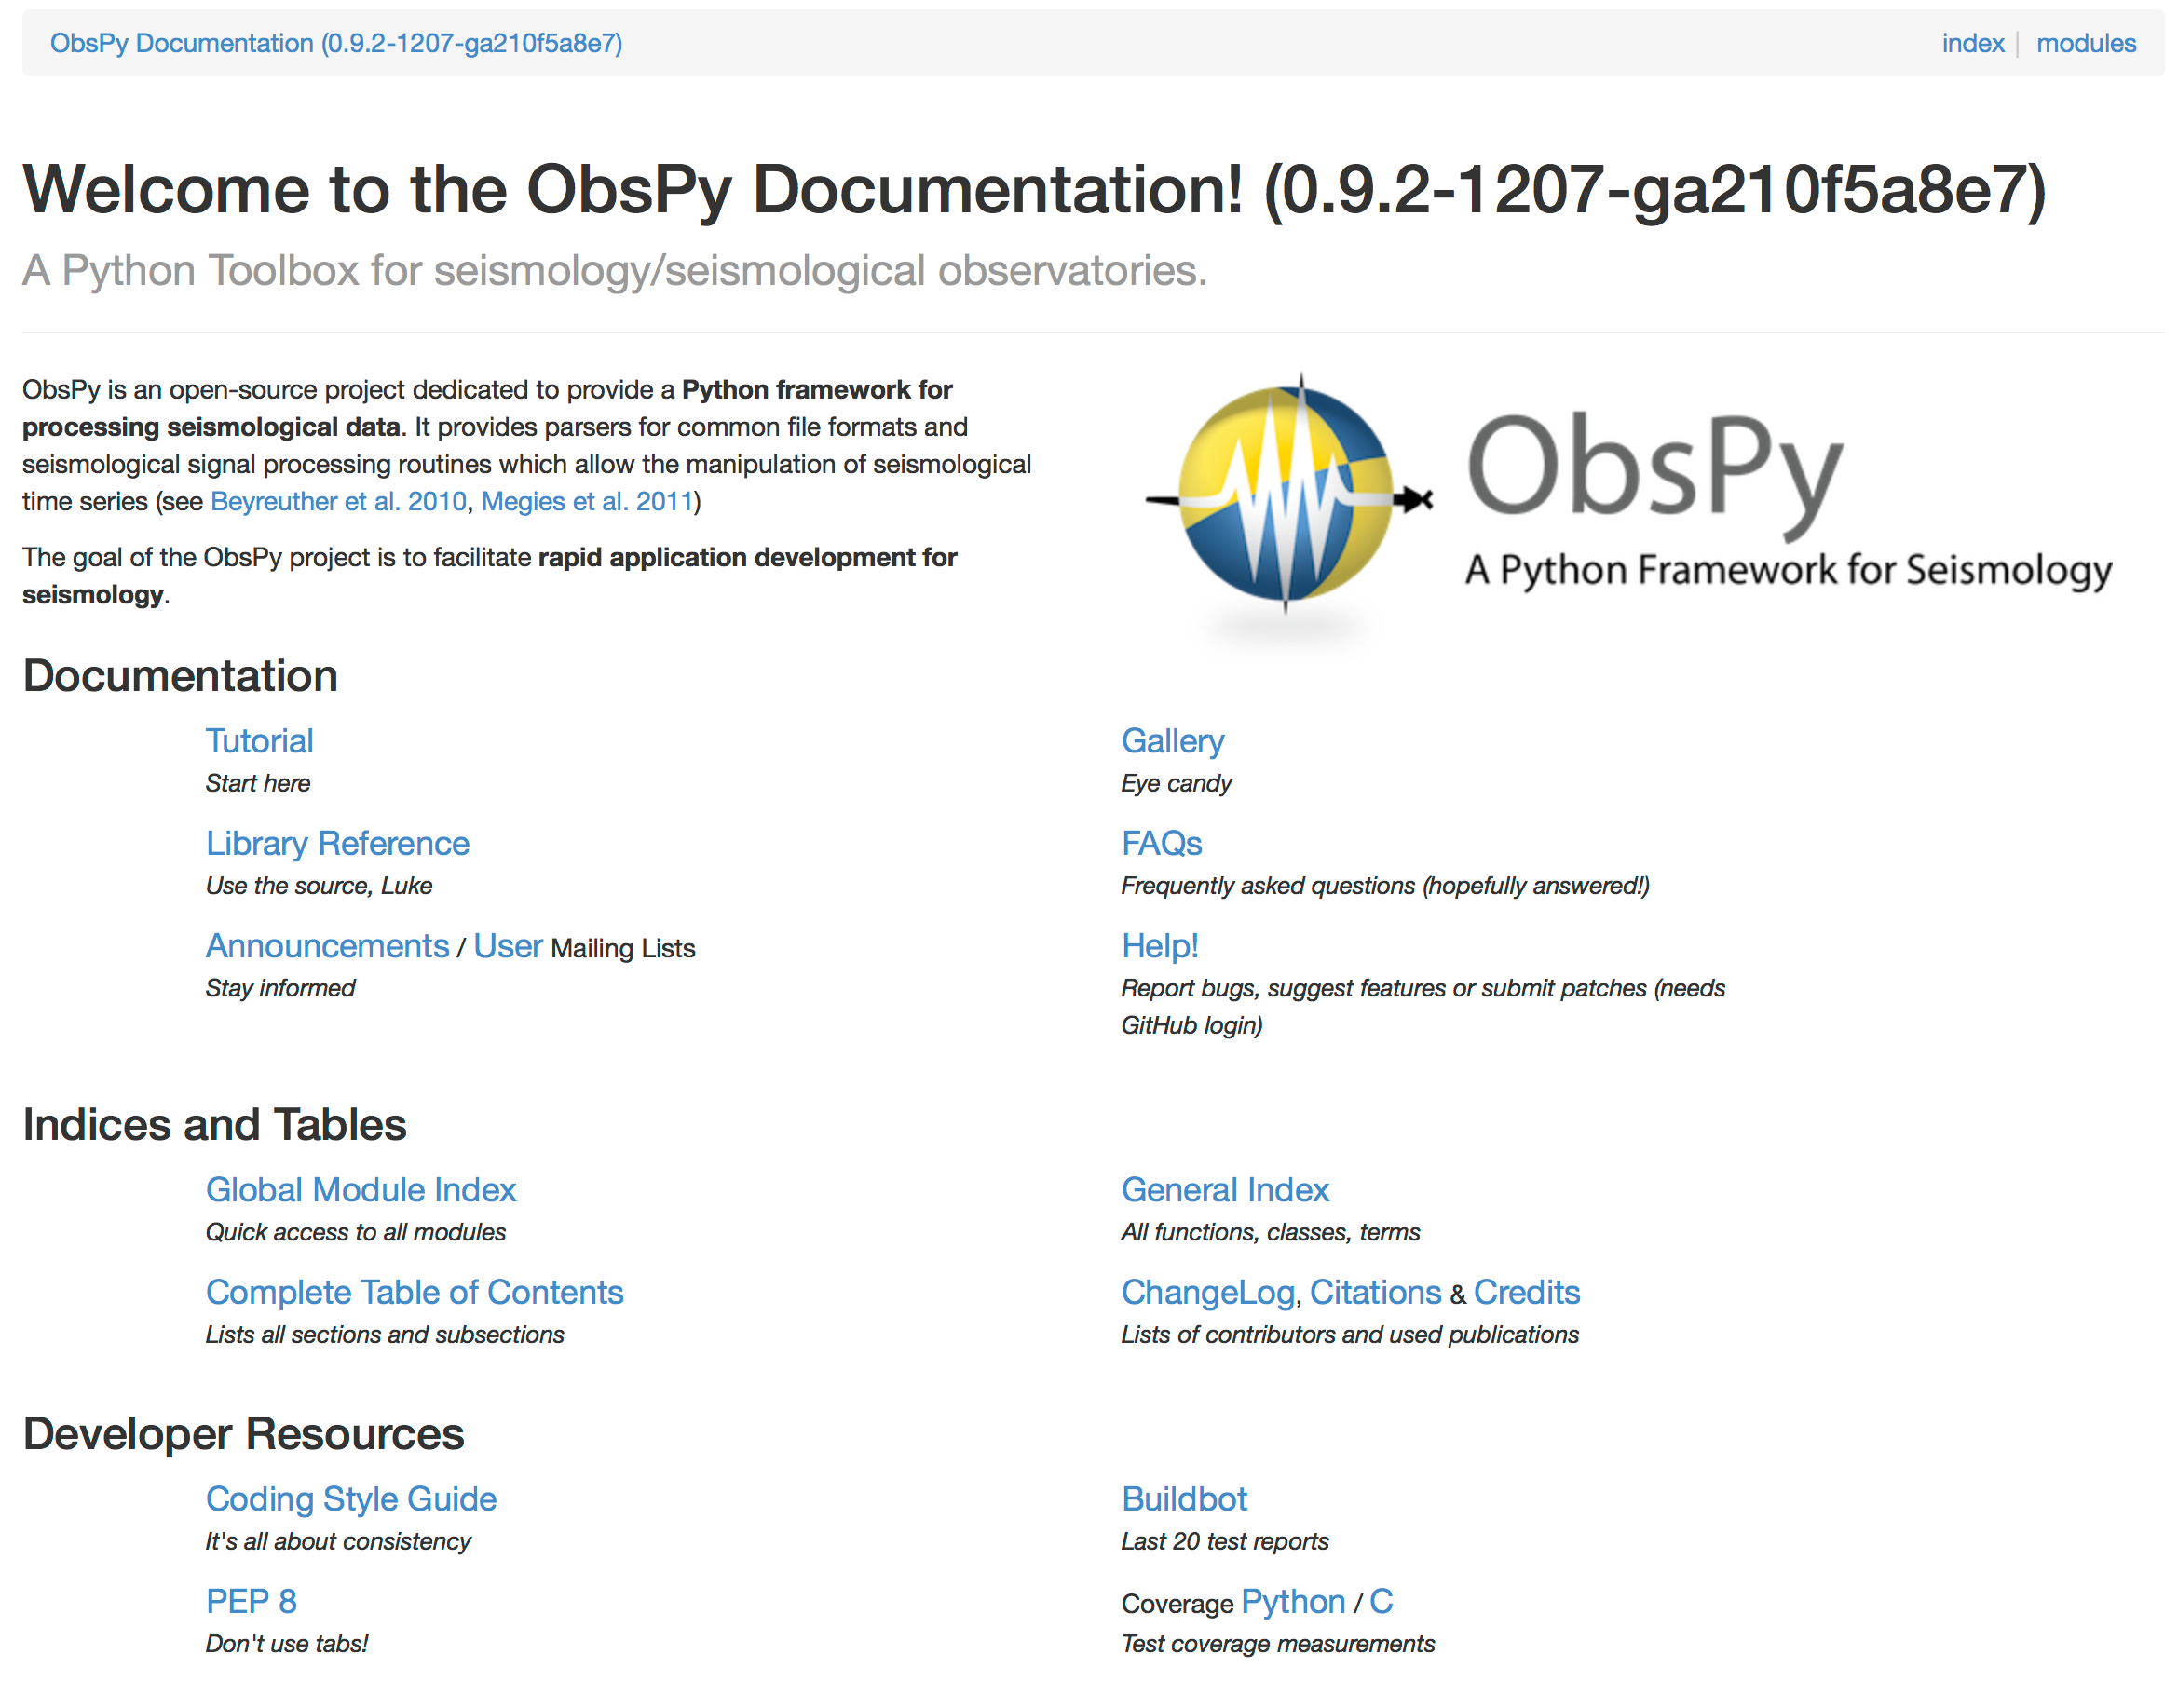
\includegraphics[width=0.7\columnwidth]{./images/website_screeny2.png}
            \end{center}
        \end{minipage}
    \end{tabularx}
    \end{center}

}\vspace{\MyBoxVSep}

\MyBox[8em]{
\section*{Why Use Python?}
\small
\begin{multicols}{2}
\begin{itemize}
    \item Easy to learn $\Rightarrow$ Learning curve similar to Matlab
    \item Free and  Open Source
    \item Cross-platform $\Rightarrow$ Runs everywhere from RaspberryPi to large supercomputers
    \item General purpose language\\(in contrast to many other tools used in science)
    \item No need to compile and interactive shell available
    %\item ``Batteries included''
    \item Mature third party libraries
    \item Easy to interact with legacy C and Fortran code

    \item One of the most used programming languages
    \item Huge community outside of science\\$\Rightarrow$ Tools and support widely available
    %\item Used a lot in the web community\\$\Rightarrow$ Will become more and more important
    %\item Big support from the data analysis community
    \item Interesting new developments: PyPy, Blaze, numba, IPython, pandas, \dots
\end{itemize}
\end{multicols}

}\vspace{\MyBoxVSep}

\MyBox[8em]{
\section*{References}
\footnotesize
B\textsc{eyreuther}, M., R. B\textsc{arsch}, L. K\textsc{rischer}, T. M\textsc{egies}, Y. B\textsc{ehr} and J. W\textsc{assermann} (2010)\\
\textbf{ObsPy: A Python Toolbox for Seismology}\\
Seismological Research Letters, 81(3):530-533, doi:10.1785/​gssrl.81.3.530\\

M\textsc{egies}, T., M. B\textsc{eyreuther}, R. B\textsc{arsch}, L. K\textsc{rischer} and J. W\textsc{assermann} (2011)\\
\textbf{ObsPy – What can it do for data centers and observatories?}\\
Annals Of Geophysics, 54(1), 47-58, doi:10.4401/ag-4838\\

K\textsc{rischer}, L., T. M\textsc{egies}, R. B\textsc{arsch}, M. B\textsc{eyreuther}, T. L\textsc{ecocq}, C. C\textsc{audron} and J. W\textsc{assermann} (2014)\\
\textbf{ObsPy: A Bridge for Seismology into the Scientific Python Ecosystem}\\
Computational Science \& Discovery, accepted

}\vspace{\MyBoxVSep}
\end{multicols}


% First reduce the vertical spacing to zero and then expand again.
\vspace{-0.60cm}
\vspace{\MyBoxVSep}

% New width.
\setlength{\MyBoxWidth}{736.5mm}
% Single Large Box, full width.
\MyBox[8em]{
\begin{multicols}{3}
\section*{The Scientific Python Ecosystem}
\small
Over the last decade, Python grew a vast and rich ecosystem of scientific third
party libraries. \textbf{ObsPy serves as a bridge} and enables its users to
effortlessly tie into this system giving access to large amounts of tools
designed to process and analyze data. This box quickly introduces the core
packages needed for scientific analysis.

\vspace{1ex}
\noindent\hrulefill
\vspace{1ex}

    \begin{center}
    \begin{tabularx}{\textwidth}{rX}
        \begin{minipage}{0.25\columnwidth}
            \begin{center}
            
\includegraphics[height=4cm]{./images/ipython.png}
            \end{center}
        \end{minipage}
        &
        \begin{minipage}{0.7\columnwidth}
            \textbf{IPython:} Enhanced Interactive Console
            \vspace{0.5ex}
            \footnotesize{
                \begin{itemize}
                    \item Powerful interactive shells (terminal and Qt-based)
                    \item A browser-based notebook with support for code, text, mathematical expressions, inline plots and other rich media
                    \item Easy to use, high performance tools for parallel computing
                \end{itemize}
            }

        \end{minipage}
    \end{tabularx}
    \end{center}

\vspace{1ex}
\noindent\hrulefill
\vspace{1ex}

    \begin{center}
    \begin{tabularx}{\textwidth}{rX}
        \begin{minipage}{0.25\columnwidth}
            \begin{center}
            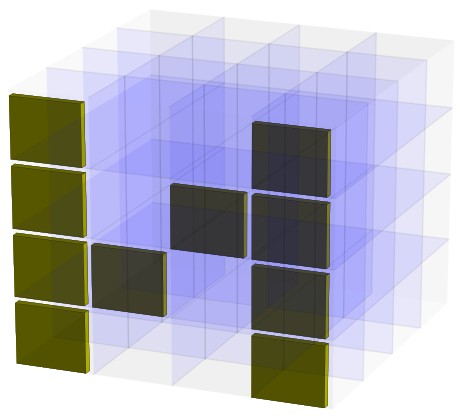
\includegraphics[height=4cm]{./images/numpy_logo.png}
            \end{center}
        \end{minipage}
        &
        \begin{minipage}{0.7\columnwidth}
            \textbf{NumPy:} \textit{Modern Array Processing}
            \vspace{0.5ex}

            \footnotesize{NumPy is the fundamental package needed for scientific
                computing with Python. Besides its obvious scientific uses, NumPy
                can also be used as an efficient multi-dimensional container of generic
                data. Arbitrary data-types can be defined. This allows NumPy to seamlessly
                and speedily integrate with a wide variety of databases.}
        \end{minipage}
    \end{tabularx}
    \end{center}

%\vspace{1ex}
%\noindent\hrulefill
%\vspace{1ex}
\columnbreak


    \begin{center}
    \begin{tabularx}{\textwidth}{rX}
        \begin{minipage}{0.25\columnwidth}
            \begin{center}
            
\includegraphics[height=4cm]{./images/scipy_med.png}
            \end{center}
        \end{minipage}
        &
        \begin{minipage}{0.7\columnwidth}
            \textbf{SciPy:} \textit{Fundamental library for scientific computing}
            \vspace{0.5ex}

            \footnotesize{SciPy is open-source software for mathematics,
                science, and engineering. It is also the name of a very popular
                conference on scientific programming with Python. The SciPy
                library depends on NumPy, which provides convenient and fast
                N-dimensional array manipulation. The SciPy library is built to
                work with NumPy arrays, and provides many user-friendly and
                efficient numerical routines such as routines for numerical
            integration and optimization.}

        \end{minipage}
    \end{tabularx}
    \end{center}

\vspace{1ex}
\noindent\hrulefill
\vspace{1ex}

    \begin{center}
    \begin{tabularx}{\textwidth}{rX}
        \begin{minipage}{0.25\columnwidth}
            \begin{center}
            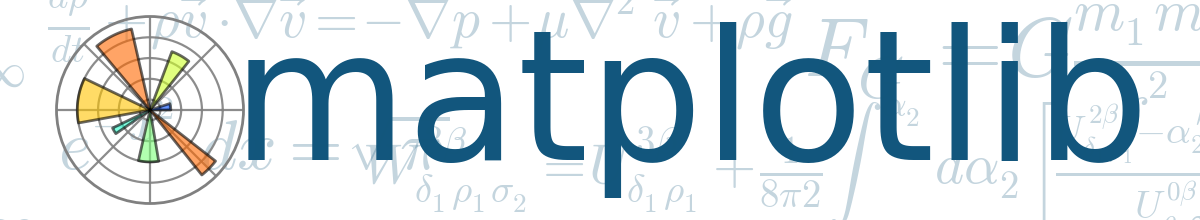
\includegraphics[width=6cm]{./images/matplotlib_med.png}
            \end{center}
        \end{minipage}
        &
        \begin{minipage}{0.7\columnwidth}
            \textbf{Matplotlib:} \textit{Comprehensive, high quality 2D Plotting}
            \vspace{0.5ex}

            \footnotesize{2D plotting library for Python that produces high
                quality figures that can be used in various hardcopy and
                interactive environments.}
        \end{minipage}
    \end{tabularx}
    \end{center}

\vspace{1ex}
\noindent\hrulefill
\vspace{1ex}

    \begin{center}
    \begin{tabularx}{\textwidth}{rX}
        \begin{minipage}{0.25\columnwidth}
            \begin{center}
            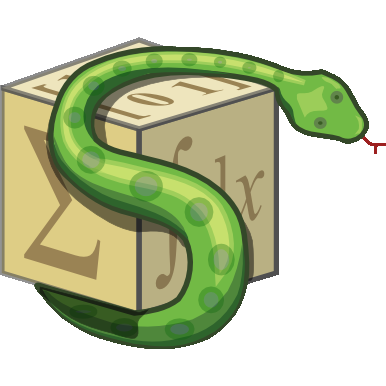
\includegraphics[height=4cm]{./images/sympy_logo.png}
            \end{center}
        \end{minipage}
        &
        \begin{minipage}{0.7\columnwidth}
            \textbf{SymPy:} \textit{Symbolic mathematics}
            \vspace{0.5ex}

            \footnotesize{SymPy is a Python library for symbolic mathematics.
                It aims to become a full-featured computer algebra system (CAS)
                while keeping the code as simple as possible in order to be
                comprehensible and easily extensible. SymPy is written entirely
                in Python and does not require any external libraries.}
        \end{minipage}
    \end{tabularx}
    \end{center}

%\vspace{1ex}
%\noindent\hrulefill
%\vspace{1ex}
\columnbreak

    \begin{center}
    \begin{tabularx}{\textwidth}{rX}
        \begin{minipage}{0.25\columnwidth}
            \begin{center}
            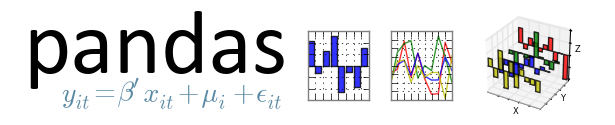
\includegraphics[width=6cm]{./images/pandas.png}
            \end{center}
        \end{minipage}
        &
        \begin{minipage}{0.7\columnwidth}
            \textbf{pandas:} \textit{Data structure \& analysis}
            \vspace{0.5ex}

            \footnotesize{pandas is a Python package providing fast, flexible, and expressive data structures designed to make working with “relational” or “labeled” data both easy and intuitive. It aims to be the fundamental high-level building block for doing practical, real world data analysis in Python. Additionally, it has the broader goal of becoming the most powerful and flexible open source data analysis / manipulation tool available in any language.}
        \end{minipage}
    \end{tabularx}
    \end{center}


\vspace{1ex}
\noindent\hrulefill
\vspace{1ex}

    \begin{center}
    \begin{tabularx}{\textwidth}{rX}
        \begin{minipage}{0.25\columnwidth}
            \begin{center}
            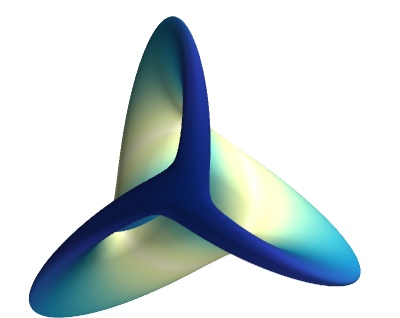
\includegraphics[width=6cm]{./images/mayavi.png}
            \end{center}
        \end{minipage}
        &
        \begin{minipage}{0.7\columnwidth}
            \textbf{Mayavi:} \textit{3D Scientific Data Visualization and Plotting}
            \vspace{0.5ex}

            \footnotesize{
                \begin{itemize}
                    \item A simple and clean scripting interface in Python, including one-liners, or an object-oriented programming interface. Mayavi integrates seamlessly with numpy and scipy for 3D plotting and can even be used in IPython interactively, similarly to Matplotlib.
                    \item The power of the VTK toolkit, harnessed through these interfaces, without forcing you to learn it.
                \end{itemize}

            }
        \end{minipage}
    \end{tabularx}
    \end{center}

\end{multicols}
}


%\setlength{\MyBoxWidth}{355mm}
%\begin{multicols}{2}
%
%\MyBox[8em]{
%\section*{website infos}
%\small


    \begin{center}
    \begin{tabularx}{\textwidth}{rX}
        \begin{minipage}{0.6\columnwidth}
\section*{ObsPy's Online Resources}
            \begin{itemize}
                \item Source Code, Bug Tracker, and Wiki
                \item Extensive documentation and example gallery
                \item Tutorial on how to get started
                \item \textbf{[obspy-users]} mailing list
                \item Installation Instructions for various platforms
                \item Use cases and user application showcases
            \end{itemize}
        \end{minipage}
        &
        \begin{minipage}{0.4\columnwidth}
            \begin{center}
%            \includegraphics[height=3cm]{./images/obspy-qr.png}
%
%            \vspace{3ex}
%
            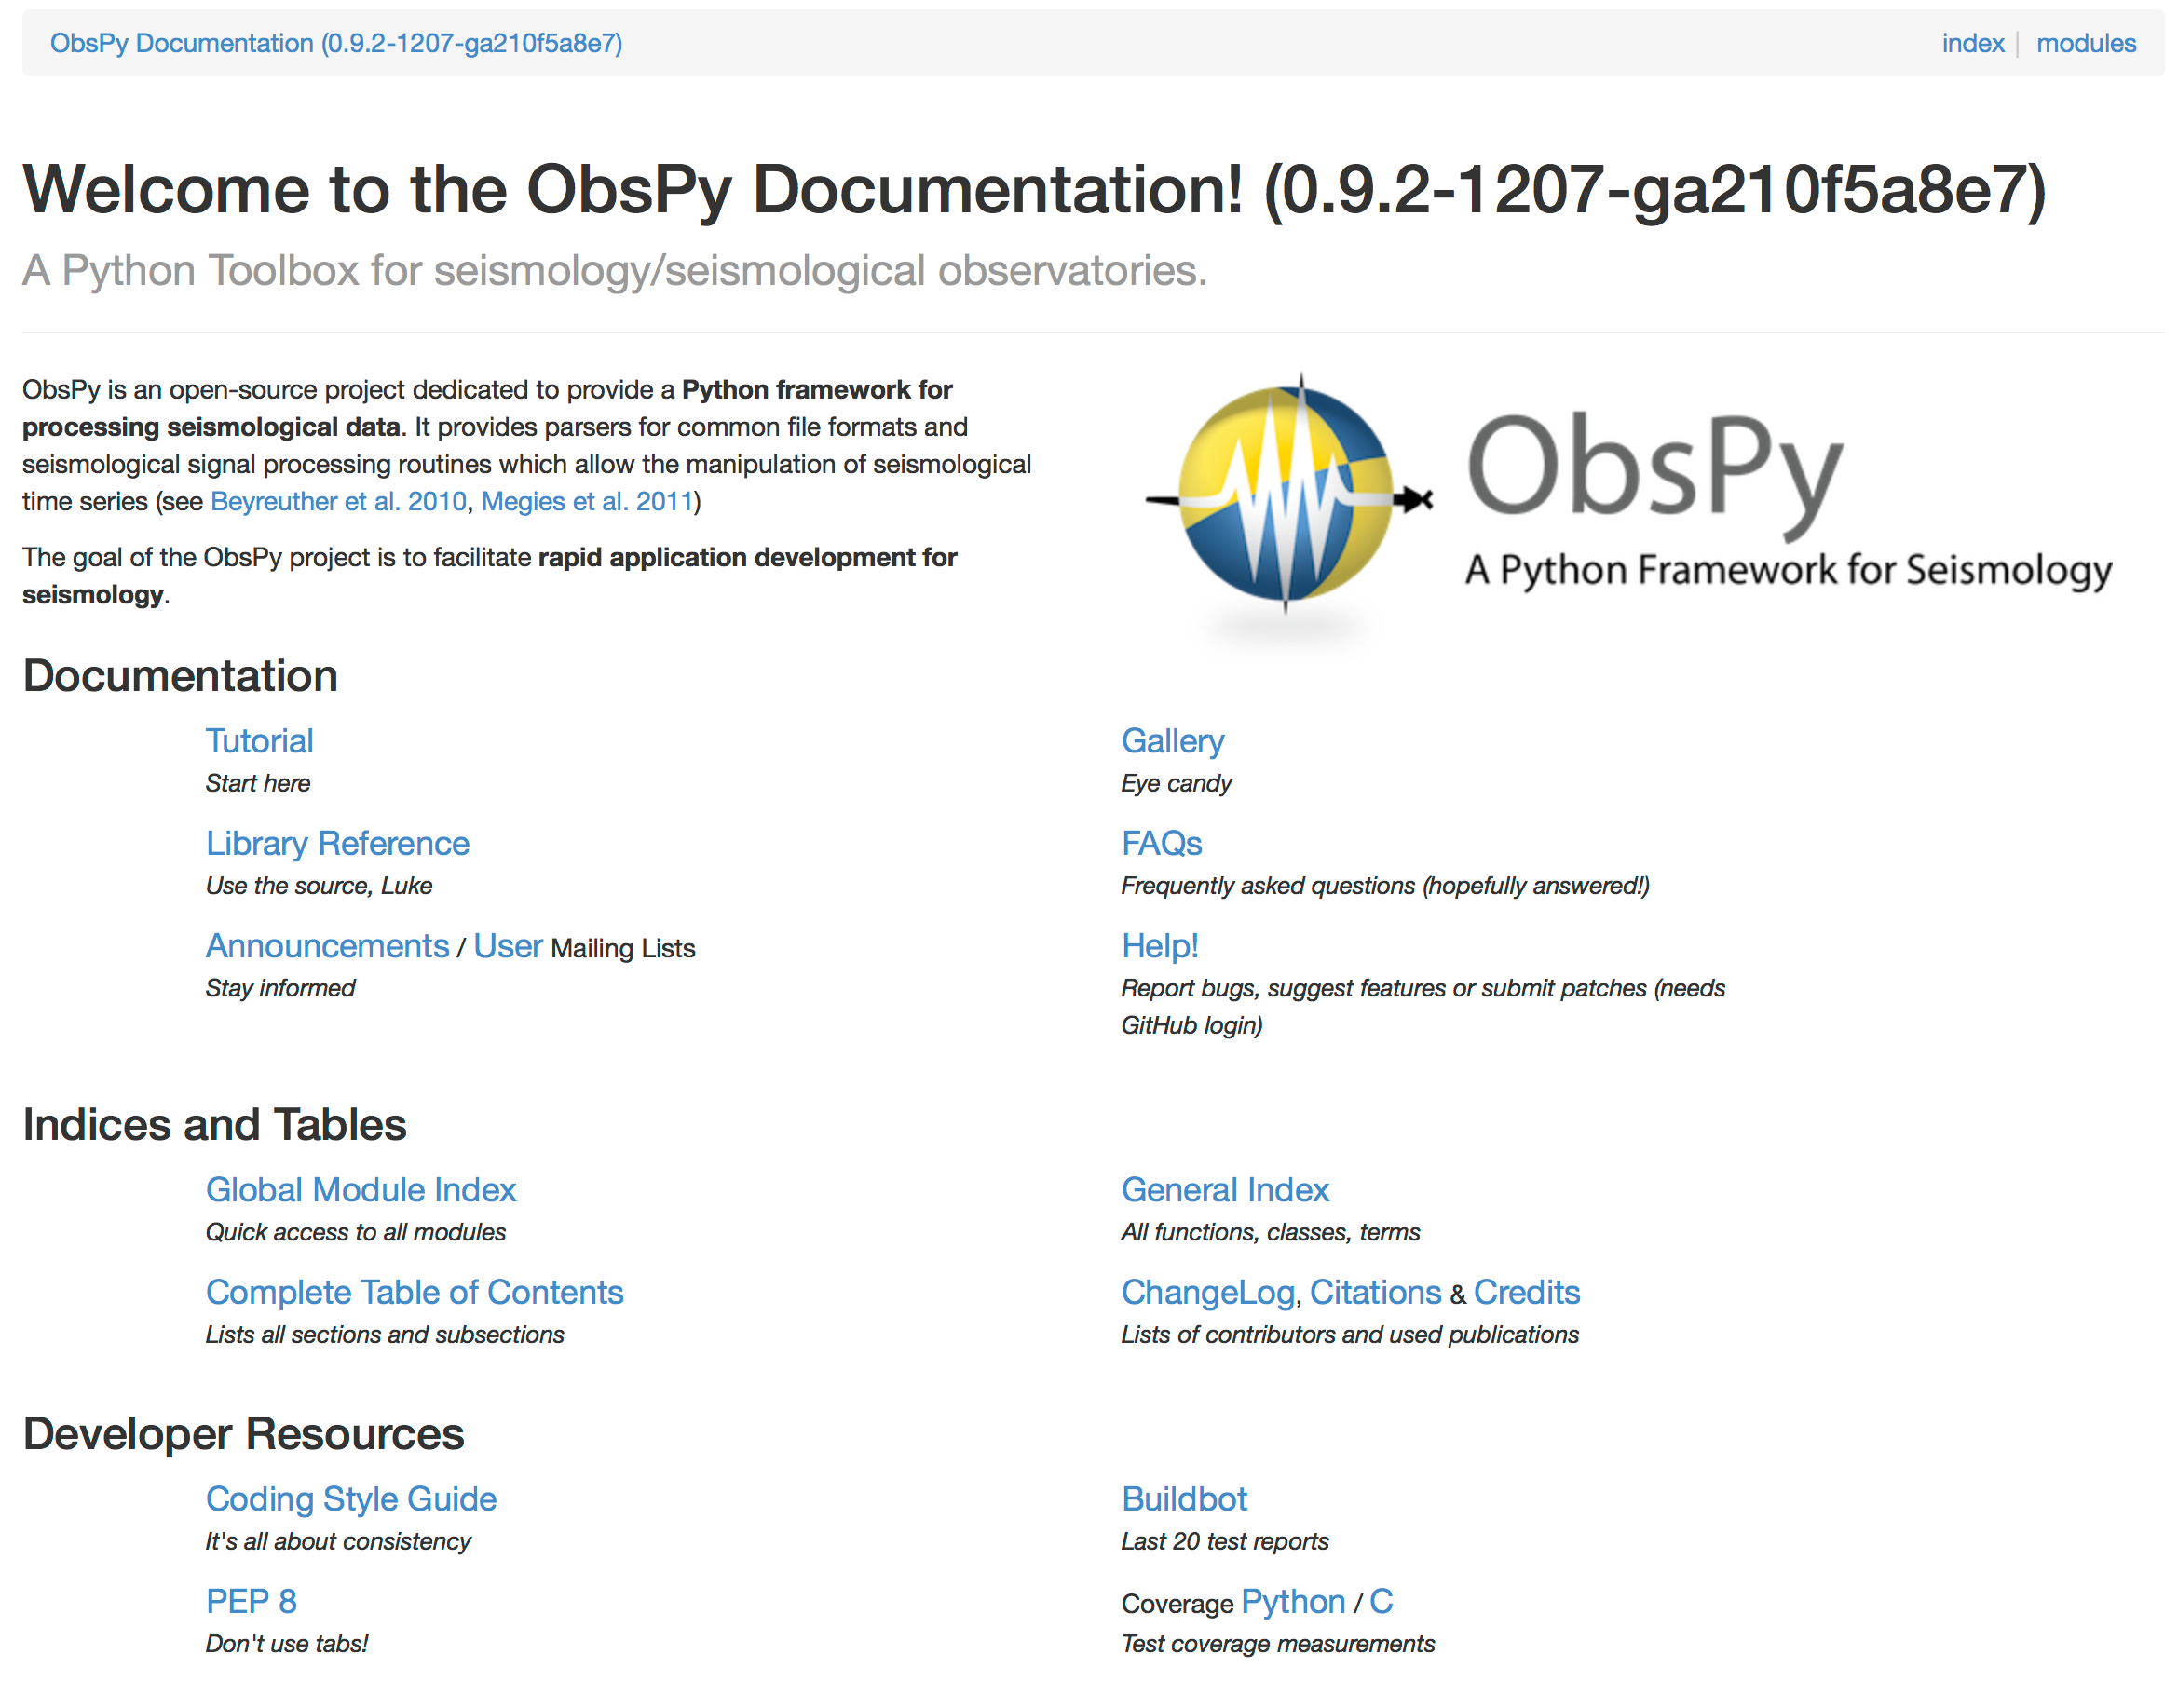
\includegraphics[width=0.7\columnwidth]{./images/website_screeny2.png}
            \end{center}
        \end{minipage}
    \end{tabularx}
    \end{center}

%}
%\columnbreak%\\
%
%\MyBox[8em]{
%\section*{References}
%\footnotesize
B\textsc{eyreuther}, M., R. B\textsc{arsch}, L. K\textsc{rischer}, T. M\textsc{egies}, Y. B\textsc{ehr} and J. W\textsc{assermann} (2010)\\
\textbf{ObsPy: A Python Toolbox for Seismology}\\
Seismological Research Letters, 81(3):530-533, doi:10.1785/​gssrl.81.3.530\\

M\textsc{egies}, T., M. B\textsc{eyreuther}, R. B\textsc{arsch}, L. K\textsc{rischer} and J. W\textsc{assermann} (2011)\\
\textbf{ObsPy – What can it do for data centers and observatories?}\\
Annals Of Geophysics, 54(1), 47-58, doi:10.4401/ag-4838\\

K\textsc{rischer}, L., T. M\textsc{egies}, R. B\textsc{arsch}, M. B\textsc{eyreuther}, T. L\textsc{ecocq}, C. C\textsc{audron} and J. W\textsc{assermann} (2014)\\
\textbf{ObsPy: A Bridge for Seismology into the Scientific Python Ecosystem}\\
Computational Science \& Discovery, accepted

%}
%\end{multicols}
%\end{document}

\end{document}

%%%%%%%%%%%%%%%%%%%%%%%%%%%%%%%%%%%%%%%%%%%%%%%%%%%%%%%%%%%%%%%%%%%%%%%%%%%%%%%%%
%%%%%%%%%%%%%%%%%%%%%%%%%%%%%%%%%%%%%%%%%%%%%%%%%%%%%%%%%%%%%%%%%%%%%%%%%%%%%%%%%
%%%%%%%%%%%%%%%%%%%%%%%%%%%%%%%%%%%%%%%%%%%%%%%%%%%%%%%%%%%%%%%%%%%%%%%%%%%%%%%%%
%%%%%%%%%%%%%%%%%%%%%%%%%%%%%%%%%%%%%%%%%%%%%%%%%%%%%%%%%%%%%%%%%%%%%%%%%%%%%%%%%
%%%%%%%%%%%%%%%%%%%%%%%%%%%%%%%%%%%%%%%%%%%%%%%%%%%%%%%%%%%%%%%%%%%%%%%%%%%%%%%%%
%%%%%%%%%%%%%%%%%%%%%%%%%%%%%%%%%%%%%%%%%%%%%%%%%%%%%%%%%%%%%%%%%%%%%%%%%%%%%%%%%
%%%%%%%%%%%%%%%%%%%%%%%%%%%%%%%%%%%%%%%%%%%%%%%%%%%%%%%%%%%%%%%%%%%%%%%%%%%%%%%%%
%%%%%%%%%%%%%%%%%%%%%%%%%%%%%%%%%%%%%%%%%%%%%%%%%%%%%%%%%%%%%%%%%%%%%%%%%%%%%%%%%
\nocite{obspy}

%
% Document header
%
\PosterHead{
	\textbf{\LARGE ObsPy: A Python Toolbox for Seismology/Seismological Observatories}\\[0.4ex]
	\textit{\Large Interactive Application and Rapid Program Development} \\[0.5ex]
	\large \underline{Lion Krischer}$^{\text{a}}$, Moritz Beyreuther$^{\text{a}}$, Robert Barsch$^{\text{a}}$, Tobias Megies$^{\text{a}}$, Yannik Behr$^{\text{b}}$, Joachim Wassermann$^{\text{a}}$\\
	$^{\text{a}}$ LMU Munich \hspace{2em}  $^{\text{b}}$ Victoria University of Wellington, New Zealand\\
	Department of Earth and Environmental Sciences (Geophysics), Ludwig-Maximilians-University Munich, Germany\\
	Contact: \textit{krischer@geophysik.uni-muenchen.de}, \textbf{https://www.obspy.org}
}

%
%\renewcommand{\capsize}{\footnotesize}
%
\setlength{\columnsep}{\MyBoxHSep}
\vspace{-1.5em}
\begin{multicols}{2}

%
% First box. Top left.
%
\MyBox[8em]{

\section*{Abstract}
\textbf{Python} enables the user to combine the advantages of a fully grown programming language with the flexibility of an interactive scripting language. Its extensive standard library and many freely available high quality scientific modules enable rapid development.

\textbf{ObsPy} provides the ability to read and write many common waveform file formats as well as seismological signal processing routines.

Furthermore \textbf{NumPy} (numpy.scipy.org) and \textbf{SciPy} (scipy.org) offer a wide variety of numerical multidimensional array programming methods. Together with \textbf{IPython} (ipython.scipy.org) and \textbf{Matplotlib} (matplotlib.sourceforge.net) ObsPy offers a powerful, text-based and easy to learn interactive environment consisting of free software packages.

ObsPy has a \textbf{modular architecture} which aims at minimizing the dependencies and is available under the \textbf{GPL/LGPLv3} licences.
}\vspace{\MyBoxVSep}


%
% Second box.
%
\MyBox[8em]{

\section*{Reading and Writing}
ObsPy provides unified access to read and write most commonly used waveform formats such as \textbf{MiniSEED, GSE2, SAC, SEISAN and the Seismic Handler formats Q and ASCII}. All data is stored in a Stream object consisting of multiple Traces of contiguous time series. Every Trace keeps track of its own meta information and the data is available as \textbf{numpy.ndarrays}.

% Code for reading.
\lstinputlisting[firstline=1, lastline=5]{code/reading.py}

The Stream and Trace objects have many built-in methods, like filtering and plotting:
\lstinputlisting[firstline=7, lastline=7, firstnumber=6]{code/reading.py}

\begin{center}
\begin{tikzpicture}
\node[above right,text width=0.9\textwidth]at(0cm,0cm){ 
\tiny
\centering
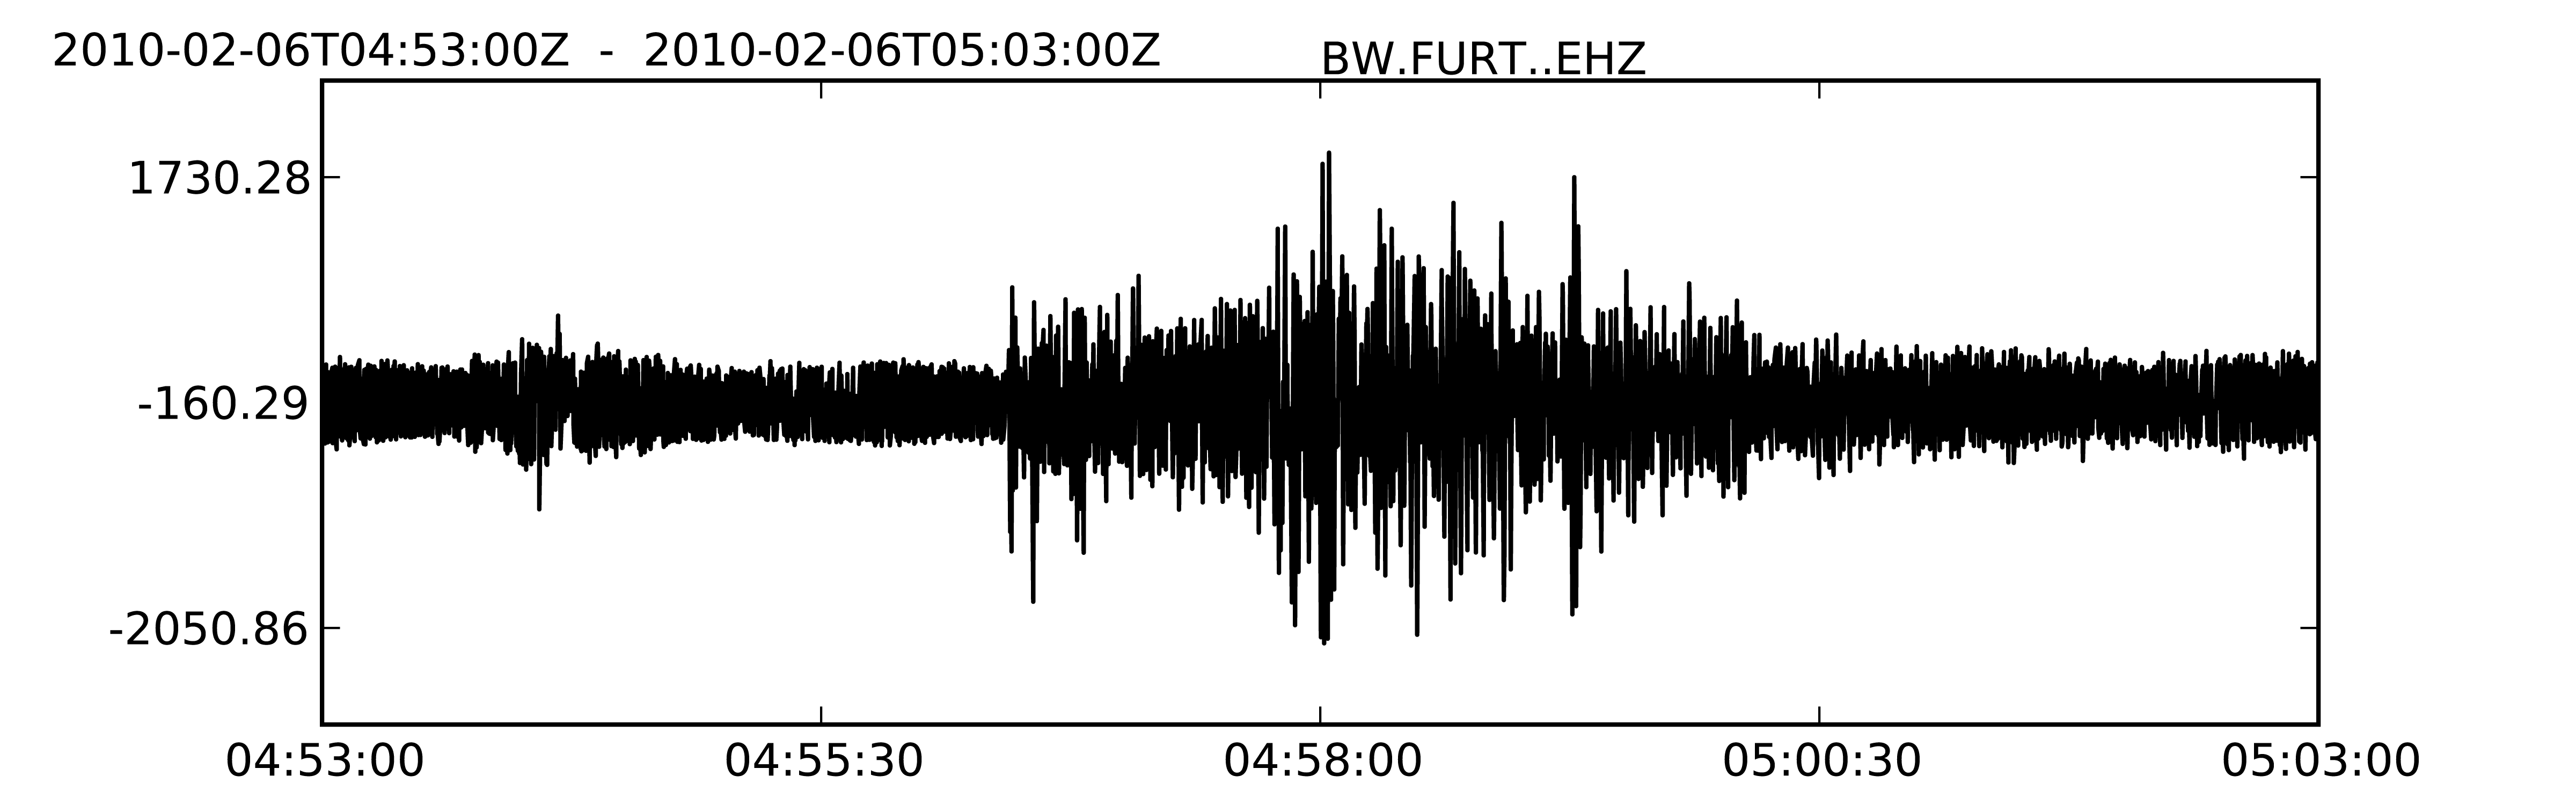
\includegraphics[width=0.9\textwidth]{simple_plot}\\[-3ex]
};
\end{tikzpicture}
{\newline \small \textbf{Figure~1}: Graphical representation of the Stream object. Created with obspy.imaging.
} \\[.5\MyBoxVSep]
\end{center}

\vspace{2ex}
Data can be exported with the write method.
\lstinputlisting[firstline=9, lastline=9, firstnumber=7]{code/reading.py}


}\vspace{\MyBoxVSep}

\MyBox[8em]{

\section*{Data Retrieval}
ObsPy also has support to retrieve data from ArcLink (www.webdc.eu), Fissures (www.iris.edu/dhi) and SeisHub (www.seishub.org)\citep{seishub}:\\
\newline
\vspace{-2ex}
\lstinputlisting[firstline=7, lastline=10, firstnumber=1]{code/arclink.py}
}\vspace{\MyBoxVSep}

\columnbreak%\\

%
% Third box.
%
\MyBox[8em]{
\section*{SEED/XML-SEED Support}
XML-SEED \citep{xseed} is a XML representation of the Dataless SEED format \citep{seed}. ObsPy is able to convert SEED
\lstinputlisting{code/seed_example.py}
to XML-SEED and back and furthermore it can extract RESP files from either format.
\lstinputlisting[firstline=2, lastline=5]{code/xseed_example.py}
\textbf{obspy.xseed} is, to the authors' knowledge, the only freely available and working implementation of XML-SEED.

}\vspace{\MyBoxVSep}

%
% Fourth box.
%

\MyBox[8em]{
\begin{multicols}{2}
\section*{obspy.signal}
Various processing routines, for example:
\vspace{-2ex}
\subsection*{Instrument Correction}
This example shows the correction of a STS2 to a 1 Hz seismometer using \textbf{obspy.signal}.
\newline
The data is read with \textbf{obspy.core}, then the mean value is subtracted.
\lstinputlisting[firstline=8, lastline=9, firstnumber=9]{code/korrektur.py}
Now the data is corrected with the simulate() method of the Trace object which calls some functions in obspy.signal. \textit{sts2} and \textit{onehzinst} are Python dictionaries containing information about the instrument responses.
\lstinputlisting[firstline=19, lastline=19, firstnumber=19]{code/korrektur.py}

\subsection*{Beamforming/FK Analysis}
One of ObsPy's newer developments is the inclusion of FK Analysis. It works on ObsPy's standard Stream and Trace objects.
% Include code.
\lstinputlisting[firstline=3, lastline=3, firstnumber=3]{code/beamforming.py}
The Trace objects can store response information and coordinates for easier handling. After the data is corrected as explained above and setting all the necessary arguments in a dictionary, the analysis can be performed with one single call.
\lstinputlisting[firstline=30, lastline=30, firstnumber=28]{code/beamforming.py}
The output can then be plotted with Matplotlib or further processing can be applied.
\columnbreak



\columnbreak
\begin{center}
\begin{tikzpicture}
\node[above right,text width=.45\MyBoxWidth]at(0cm,0cm){ 
\tiny
\centering
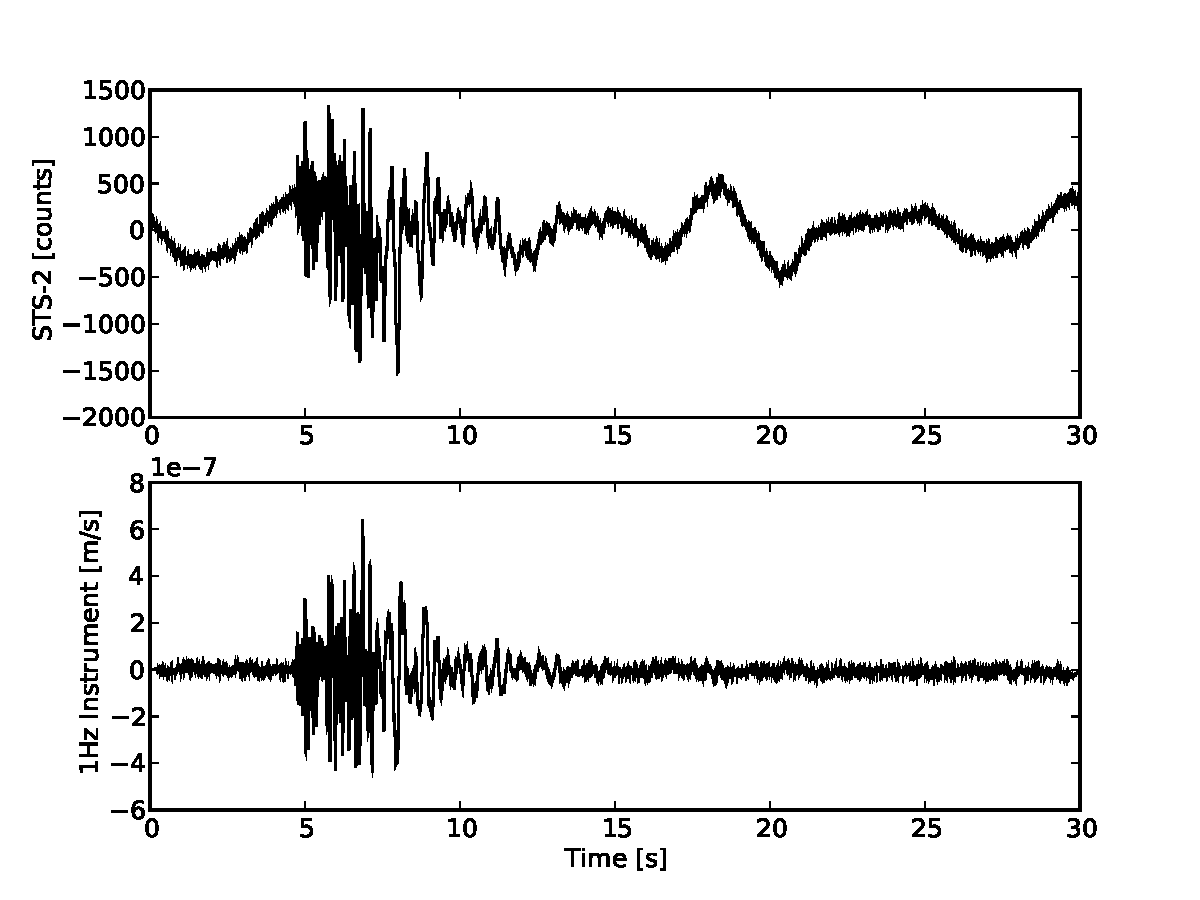
\includegraphics[height=.30\MyBoxWidth]{korrektur}\\[-3ex]
};
\end{tikzpicture}
	{\small
	\textbf{Figure~2}: Correction of a STS2 to a 1Hz instrument.
	} \\[.5\MyBoxVSep]
\end{center}

\begin{center}
\begin{tikzpicture}
\node[above right,text width=.45\MyBoxWidth]at(0cm,0cm){ 
\tiny
\centering
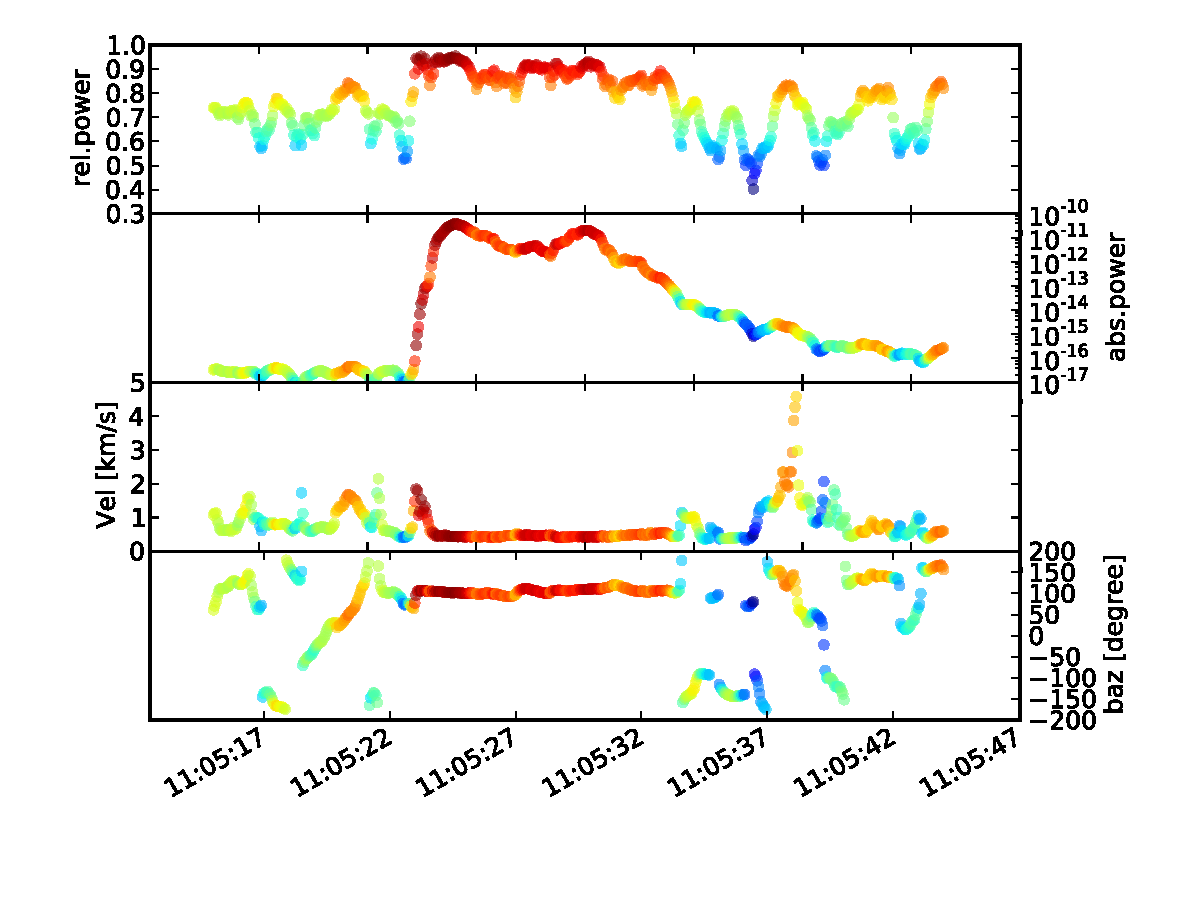
\includegraphics[height=.30\MyBoxWidth]{beamforming2}\\[-3ex]
};
\end{tikzpicture}
	{\small
	\textbf{Figure~3}: Output of a FK Analysis from blasting the AGFA skyscraper in Munich. Colors correspond to relative power.
	} \\[.5\MyBoxVSep]
\end{center}

\begin{center}
\begin{tikzpicture}
\node[above right,text width=.45\MyBoxWidth]at(0cm,0cm){ 
\tiny
\centering
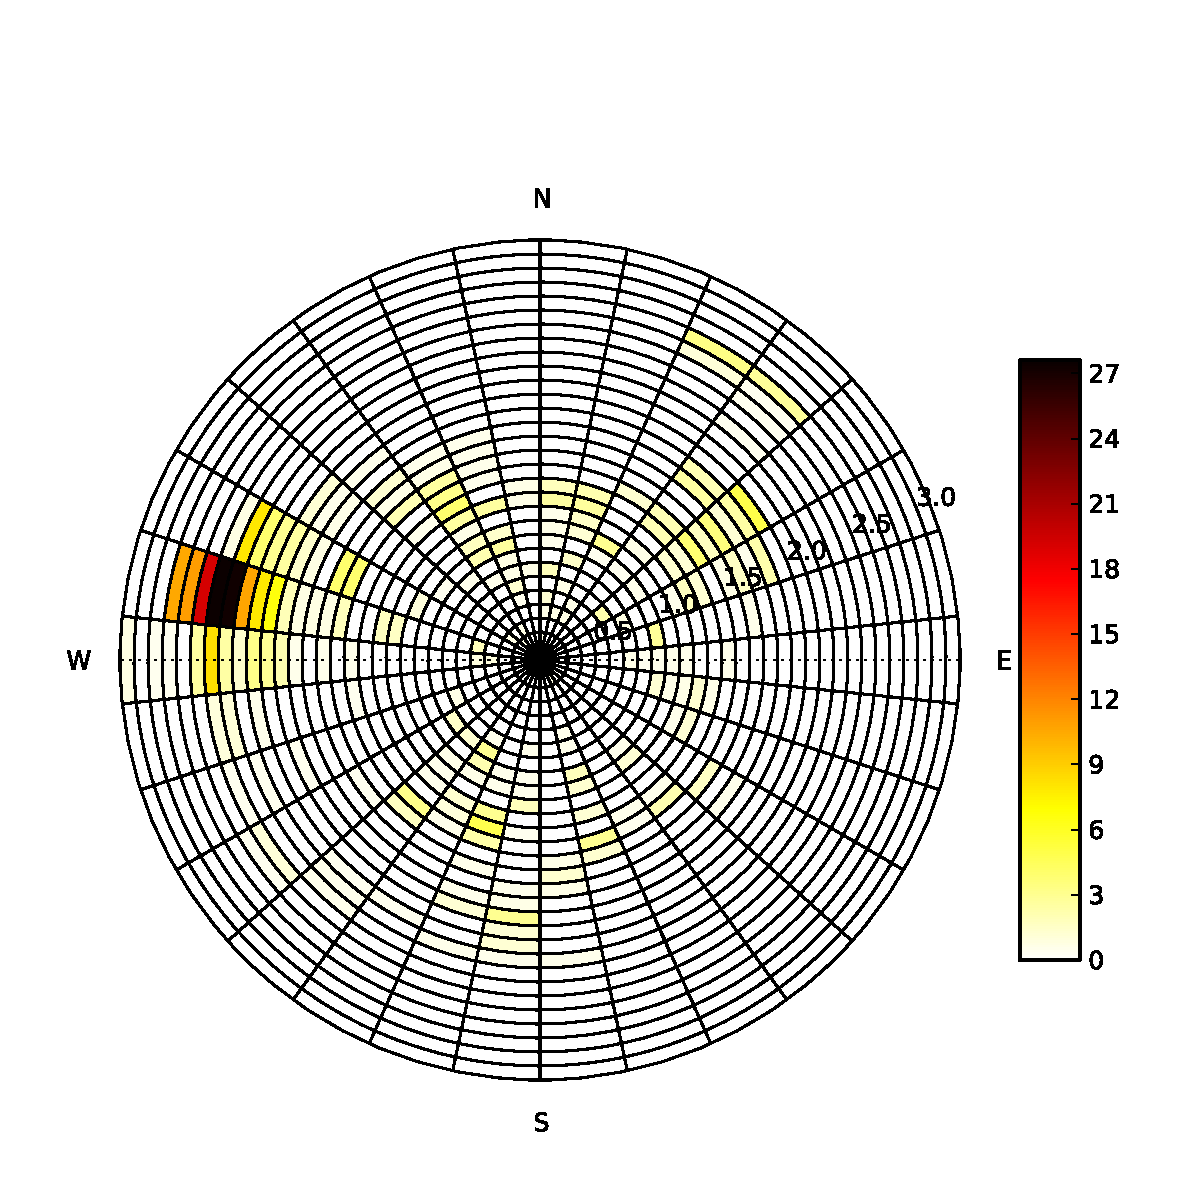
\includegraphics[height=.30\MyBoxWidth]{fkanalysis}\\[-3ex]
};
\end{tikzpicture}
	{\small
	\textbf{Figure~4}: Polar plot of the same FK Analysis.
	} \\[.5\MyBoxVSep]
\end{center}
\end{multicols}
}\vspace{\MyBoxVSep}

\end{multicols}
% First reduce the vertical spacing to zero and then expand again.
\vspace{-0.60cm}
\vspace{\MyBoxVSep}

% New width.
\setlength{\MyBoxWidth}{736.5mm}
% Single Large Box to take care of the example.
\MyBox[8em]{
\begin{multicols}{3}
\section*{Applications Using ObsPy}
Combining Python and ObsPy facilitates the development of applications ranging from little helper scripts to full blown platform-independent GUI applications with complex workflows.\\
This section highlights two GUI programs both based on Qt (qt.nokia.com) for the graphical representation. Both were developed in a matter of a few month and make use of ObsPy for the underlying internal data storage which in turn enables them to utilize ObsPy's routines for many commonly used tasks, e.g. filtering and instrument simulation and they instantly gain the ability to work with most commonly used waveform dataformats.\\
Other advanced third party Python modules that are easily integrated can take care of most processing and plotting needs so the programmer can focus on creating unique new features.\\
An up to date list of programs making use of ObsPy is available at www.obspy.org. A notable example is the newly developed version of \textbf{SeismicHandler} (www.seismic-handler.org) which is also represented at this meeting.
\columnbreak
\begin{center}
\begin{tikzpicture}
\node[above right,text width=.17\MyBoxWidth]at(0cm,0cm){ 
\tiny
\centering
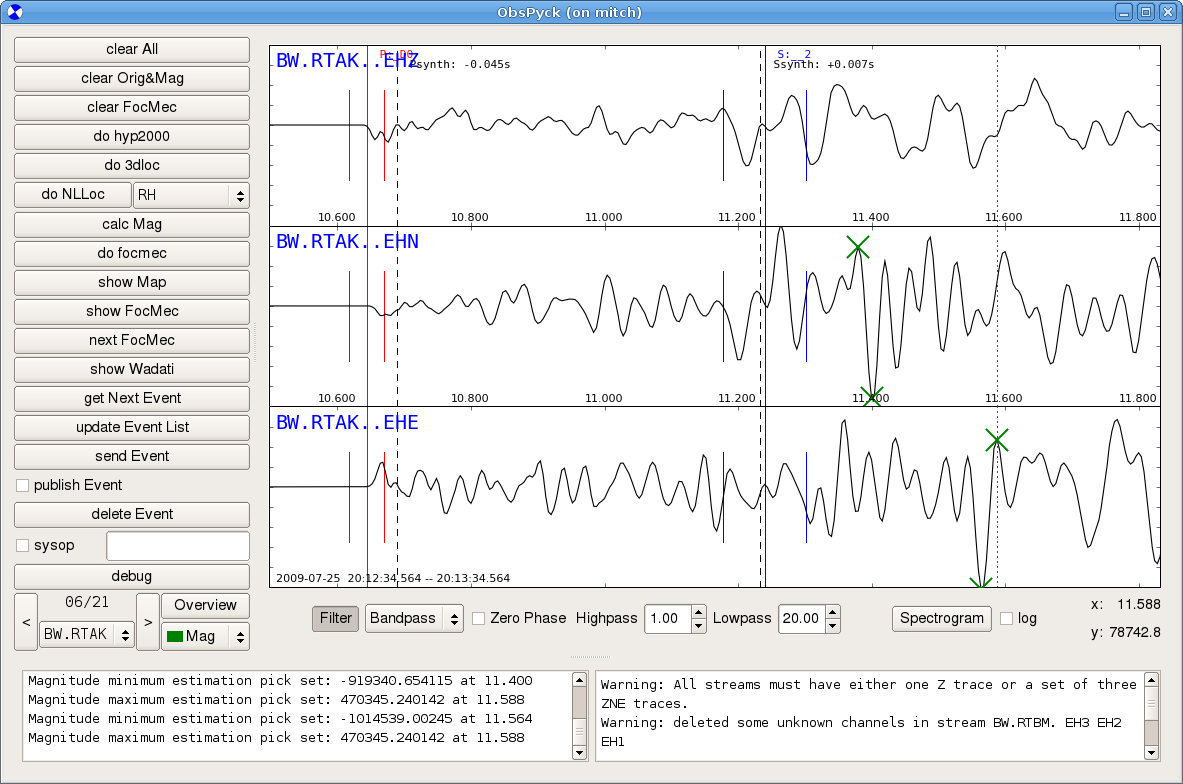
\includegraphics[height=.17\MyBoxWidth]{all_picks}\\[-3ex]
};
\end{tikzpicture}
{\newline \small \textbf{Figure~5}: ObsPyck
} \\[.5\MyBoxVSep]
\end{center}

\textbf{ObsPyck} is able to perform daily routine analysis at an observatory like phase picking and locating events. All data is read and written back to one central SeisHub database server and it just recently was extended to fetch data from ArcLink and Fissures servers to integrate external data into the localization process.
\columnbreak
\begin{center}
\begin{tikzpicture}
\node[above right,text width=.17\MyBoxWidth]at(0cm,0cm){ 
\tiny
\centering
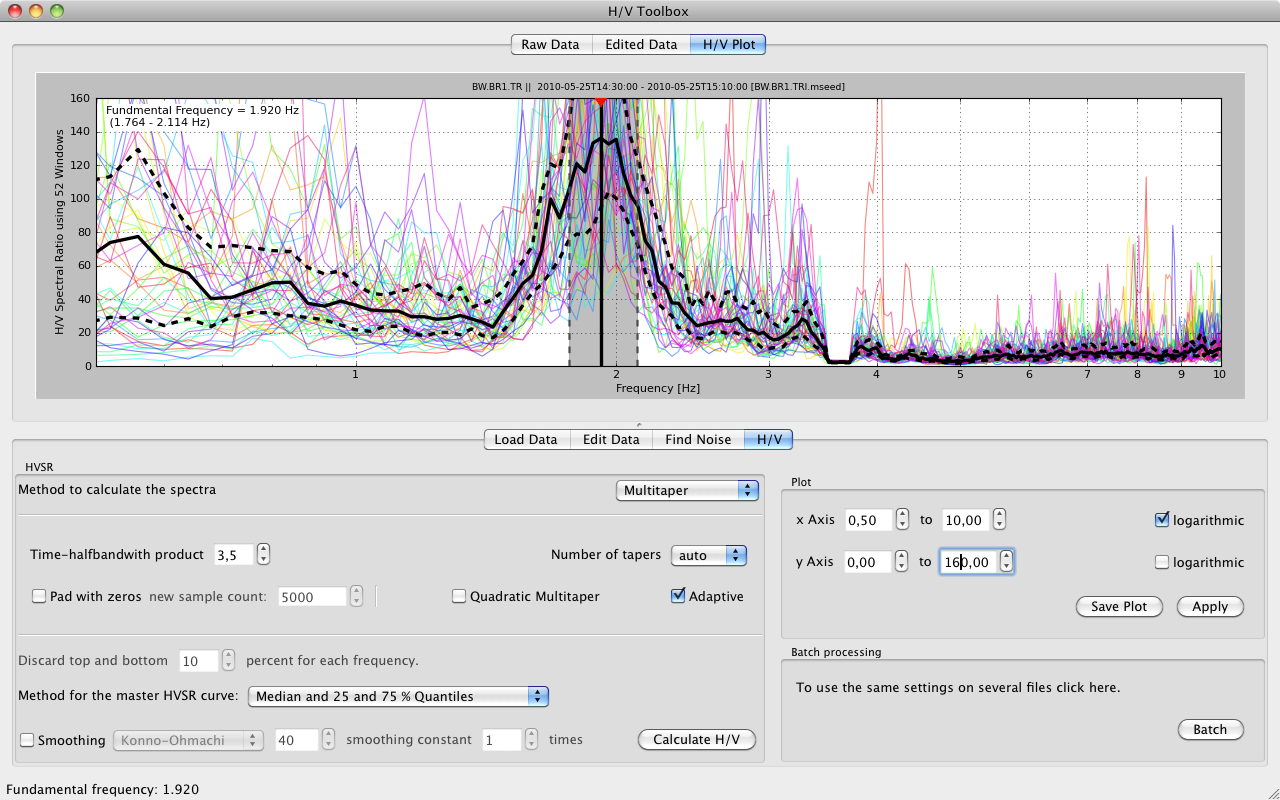
\includegraphics[height=.17\MyBoxWidth]{htovtoolbox}\\[-3ex]
};
\end{tikzpicture}
{\newline \small \textbf{Figure~6}: H/V Toolbox
} \\[.5\MyBoxVSep]
\end{center}
The \textbf{H/V Toolbox} handles the whole workflow for calculating horizontal to vertical spectral ratios (HVSR): From reading and preprocessing the data to the automated selection of appropriate time windows with little seismic activity to finally calculating the HVSR in an easy to use interface while giving visual feedback, step by step.




\end{multicols}
}

\setlength{\MyBoxWidth}{355mm}
\begin{multicols}{2}

\MyBox[8em]{
\section*{Further Information: https://www.obspy.org}
The homepage of the project \textbf{https://www.obspy.org} contains extensive \textbf{documentation}, tutorials, installation instructions for various platforms, and many more examples.
\newline
Contact the developers for support or feedback, to report bugs or to request a new feature. Contributions are more than welcome, see the developer links on the homepage if you are interested.
\newline

\underline{\textbf{Further functionality and information:}}
\begin{itemize}
\item \textbf{obspy.signal:} Filters, triggers, instrument correction, rotation, array analysis, beamforming.
\item \textbf{obspy.imaging:} Imaging spectrograms, beachballs and waveforms.
\item \textbf{Test-driven development (TDD):} TDD and automated unit tests are used throughout the ObsPy code base to ensure a high quality. Automated build bots test the most current ObsPy build on a daily basis on multiple platforms.
\end{itemize}
}
\columnbreak%\\

%
% Ninth box.
%
\MyBox[8em]{
\section*{Literature}
\vspace{2mm}
\bibliography{poster}{}
\bibliographystyle{plaindin}
}
\end{multicols}
